\chapter{GPU Implementations}
\label{chap:imp}

In this chapter, all GPU implementations will be explained in detail, both the preliminary studies done to motivate the algorithmic choices made in WARP and of those in WARP itself.

\section{Preliminary Studies}
\label{sec:prelim}

Before any serious coding efforts were undertaken, a pair of smaller preliminary studies were done to determine the feasibility of doing Monte Carlo neutron transport on GPUs.  The first study was attempting to to perform a simple, 2D, mono-energetic scattering game on a GPU.  The second study was a test of the OptiX framework to see if it could handle randomized ray tracing and still have acceptable performance.

\subsection{2D Scattering Game}

\begin{figure}[h!] 
  \centering
    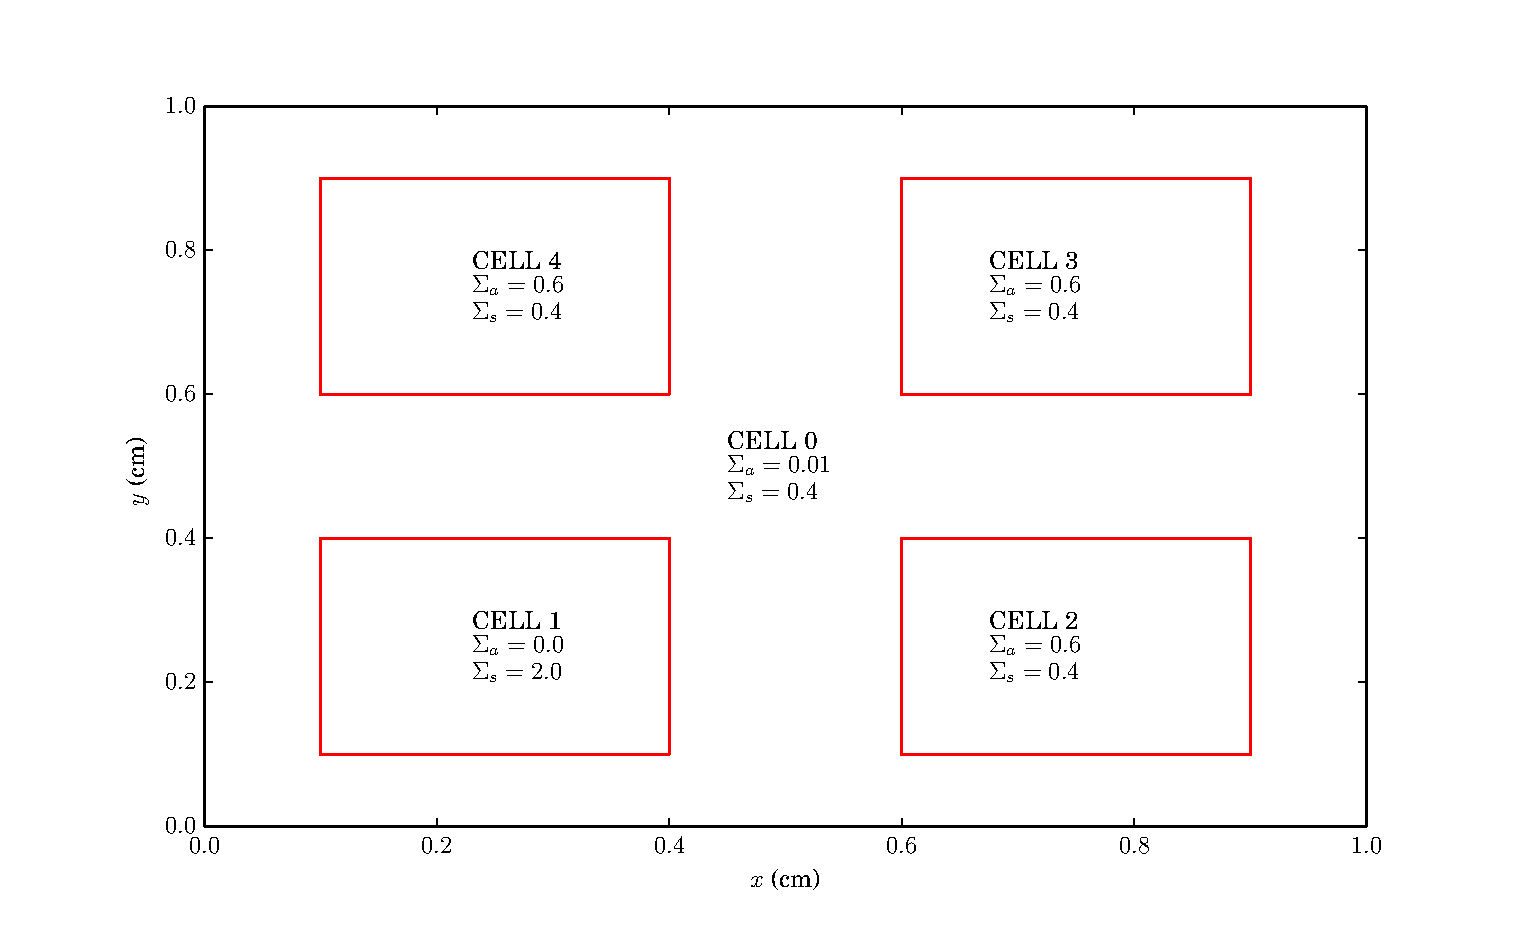
\includegraphics[width=0.8\textwidth]{graphics/prelim_geom.eps}
     \caption{The 2D geometry of the scattering test. \label{prelim_geom} }
\end{figure}

The goal of the 2D mono-energetic scattering game was to highlight if a sorted or unsorted event-based algorithm was best for controlling thread divergence on a GPU, to the see the relative performance of the history- and event-based GPU implementations to an identical serial CPU version, and to determine if the performance of the CUDPP (CUDA Parallel Primitives) library is adequate for use in WARP.   A set of three GPU implementations were written using CUDA C, and a single CPU implementation was written using C.

In the simulation, only two reaction types are possible - scattering and absorption.  Scattering is treated isotropically, and since it is mono-energetic, scattering only serves to change the direction of a particle.  The geometry of the game is simple in order to highlight how the reaction divergence is handled rather than how geometry routines effect performance.   The geometry used in the game is shown in Figure \ref{prelim_geom}.  There are five different cells, which are all square, and particles can only move in the $x$-$y$ plane.  Each cell has different reaction cross sections, and cell 0 extends to infinity, but has a nonzero absorption cross section so particles cannot scatter forever.  Particles are initialized with a uniform, random distribution in cell 1, which has no absorption cross section so they must cross a cell boundary at least once.  Since the cells are few and square, the ``where am I?'' operation that determines the cell number (and therefore the cross sections) each particle is in can be done with simple, hardcoded logic comparisons.

As particles scatter, they start to be absorbed and their histories are terminated.  This means they are no longer transported, and their data should no longer be accessed.  Here is where the GPU implementations start to differ from one another.  The task-based implementation performs the transport from a one particle per thread standpoint.  When the transport kernel is launched, each thread contains a while-loop that transports a particle until it terminates and the thread returns.  If more histories are requested than the maximum thread number, transport is performed in batches.  The diagram of the simple task-based algorithm used is shown in Figure \ref{prelim_alg_task}.  The CPU version of the code also uses this algorithm.

\begin{figure}[h!] 
  \centering
    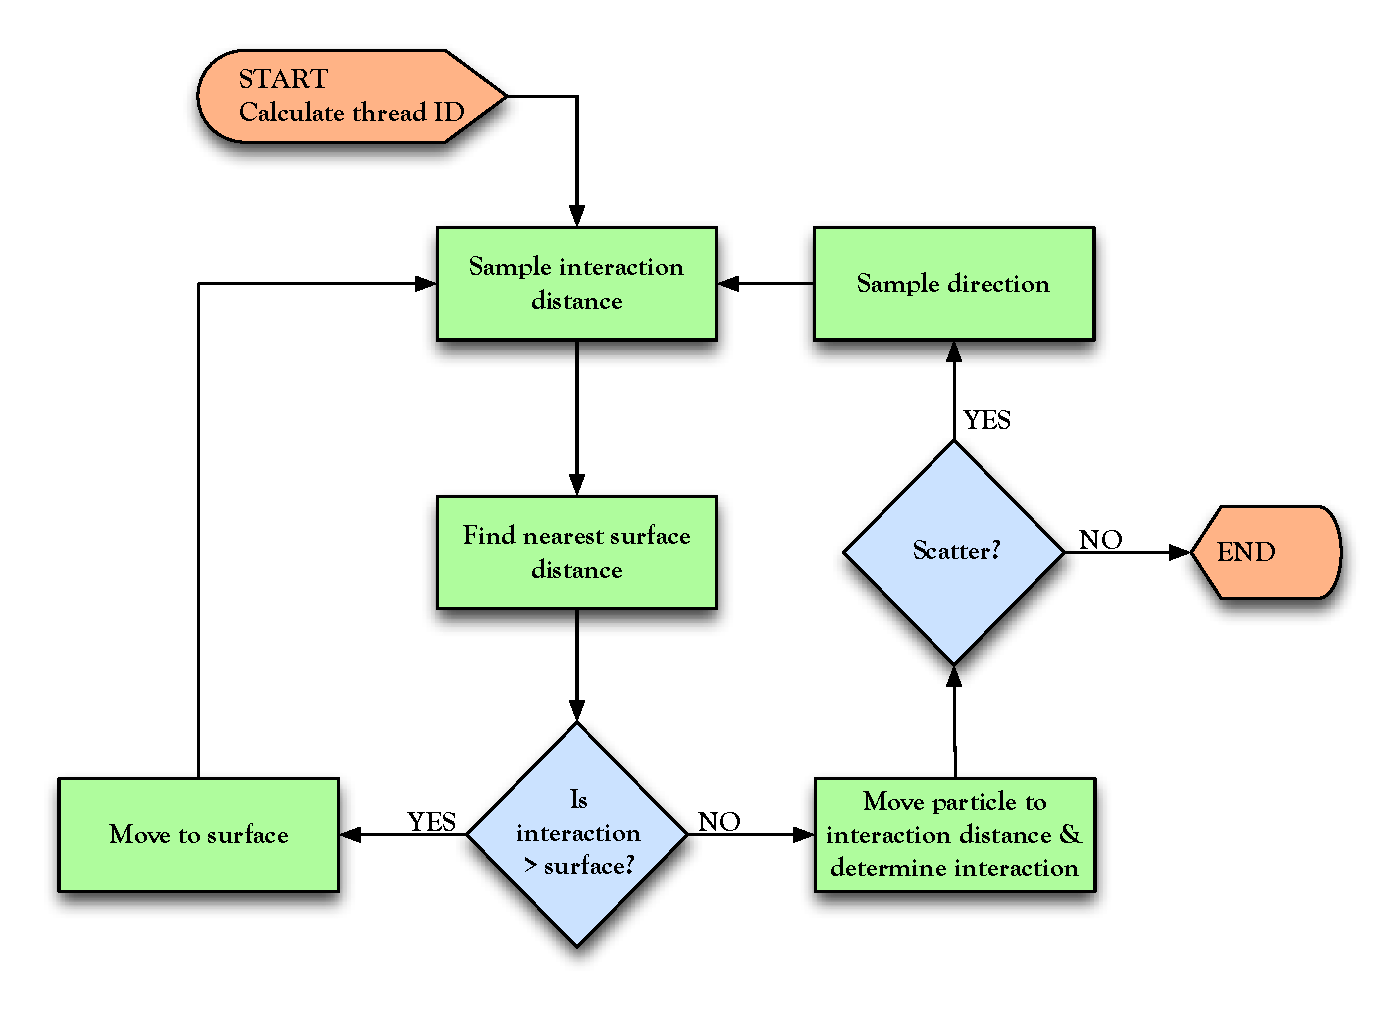
\includegraphics[width=0.7\textwidth]{graphics/prelim_alg_task.eps}
     \caption{The task-based algorithm used in the 2D scattering study. \label{prelim_alg_task} }
\end{figure}

The event-based algorithm performs the same operations on the data as the task-based algorithm, of course, but the operations are now carries out over all the particle data simultaneously in parallel.  Now, each kernel does \emph{not} contain a while loop.  The while loop is now on the CPU host, the drawbacks to which are discussed later.  Each kernel performs a single, simple task on the entire particle dataset in one step.  An analogy can be made with homework grading.  The task-based algorithm is like grading a single student's homework in its entirety, then moving on to the next student's.  The event-based approach is like grading a single \emph{problem} for \emph{every student}, then moving on to the next problem.  This makes the transport loop \emph{data parallel}, which GPUs need to keep warps coherent. 

\begin{figure}[h!] 
  \centering
    \includegraphics[width=0.7\textwidth]{graphics/prelim_alg_event.eps}
     \caption{The event-based algorithm used in the 2D scattering study. \label{prelim_alg_event} }
\end{figure}

Two different implementations were made using a event-based algorithm, one which uses the CUDPP compaction to remap threads to non-terminated (active) data, and one which does not.  In the non-remapping version, threads simply return if they access data belonging to a terminated particle.  In the remapping version, the number of threads launched is equal to the number of active particles left in the dataset, not the size of the dataset itself.  They access a remapping vector, which transforms their thread ID to be one which still contains active data.  Figure \ref{remapping} shows how the remap vector transforms the initial thread ID to an active ID.  The CUDPP compaction function does just this - it takes an input vector and a valid flag vector and returns a new vector containing only the valid elements, preserving the order which they are in.  For this test, the input vector is the thread ID vector (tid[i]=i), and the flag vector contains a 1 if a particle is unterminated and a 0 if it is not.  The compact function then returns a remapping vector which is as long as the number of unterminated particles which contains the indices of the unterminated data.

\begin{figure}[h!] 
  \centering
    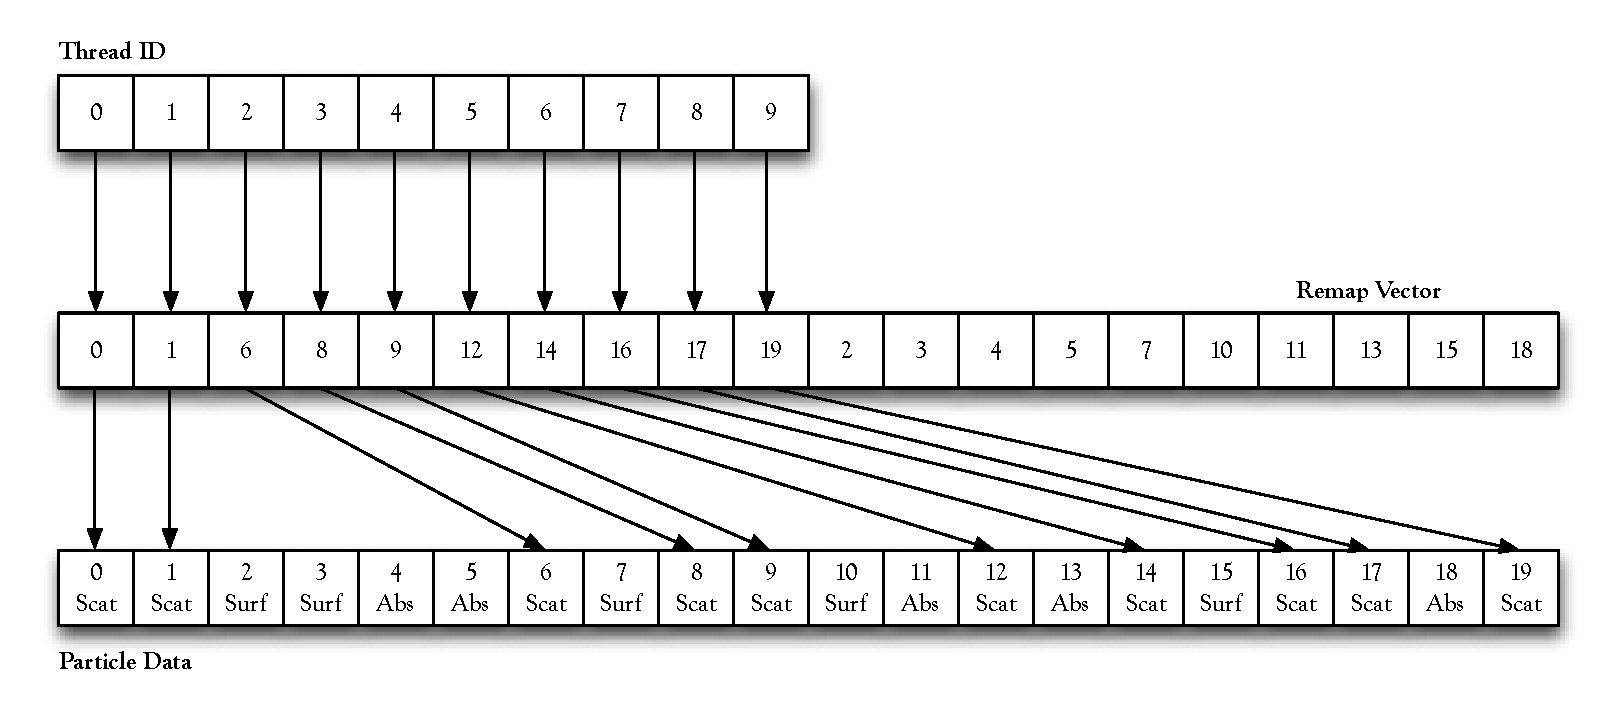
\includegraphics[width=0.8\textwidth]{graphics/remapping_horiz.eps}
     \caption{Mapping thread IDs to active data through a remapping vector \label{remapping} }
\end{figure}

Figure \ref{prelim_speedup} shows the speedup factors, $F_s=t_\mathrm{CPU}/t_\mathrm{GPU}$, of the GPU implementations over the CPU implementation versus the number of particles run.  This benchmark was run on a server with a 8-core AMD Opteron 6128 CPU clocked at 2.0GHz, and there different NVIDIA cards - a Tesla K20, a Tesla C2075, and a GeForce 480 GTX.  The following results were obtained from running the GPU implementations on the Tesla K20.  The task-parallel implementation performs best, with a maximum speedup of around 29x.  The remapping implementation has the next best performance, with about a 20x speedup over the CPU.  It's performance plateaus, unlike the batched event-based implementation.  It's performance departs from the remapping implementation at $10^5$ particles and even starts to deteriorate between $10^6$ and $10^7$ particles.  This is due to the transport having to be done in batches at this point.  The simulations were done on a Tesla C2075 card, which has Fermi architecture and a maximum block number of 65,536 for a 1D grid.  Multiplying this by 128 or 512 threads per block gives maximum total number of threads of 8,388,608 and 33,554,432, respectively.  These numbers are where the batching implementation must break the transport into multiple batches.  This is also where the task-based implementation must break transport into batches, but the effect is unnoticeable since it only implies a second kernel launch instead of hundreds more.  This limit was lifted in devices with compute capability of 3.0 and up, where the maximum 1D grid size was increased to ($10^{27}-1$) \cite{cuda}.  The speedup plot also shows another important feature - that speedup plateaus at a large number of histories.  This is due to the car'd ability to hide memory latencies through pipelining when there are many many active threads.  

The number of threads per block seems to make little difference in the event-based implementations, but makes a very large difference in the task-based implementation.  Increasing the number of threads per block from 128 to 512 reduces the performance from a 28x speedup to a 20x speedup, comparable to the event-based implementations.  The reason for this happening is most likely registers spilling to local memory since there are more threads resident in a multiprocessor and more variables need to be stored in the registers.

\begin{figure}[h!] 
  \centering
    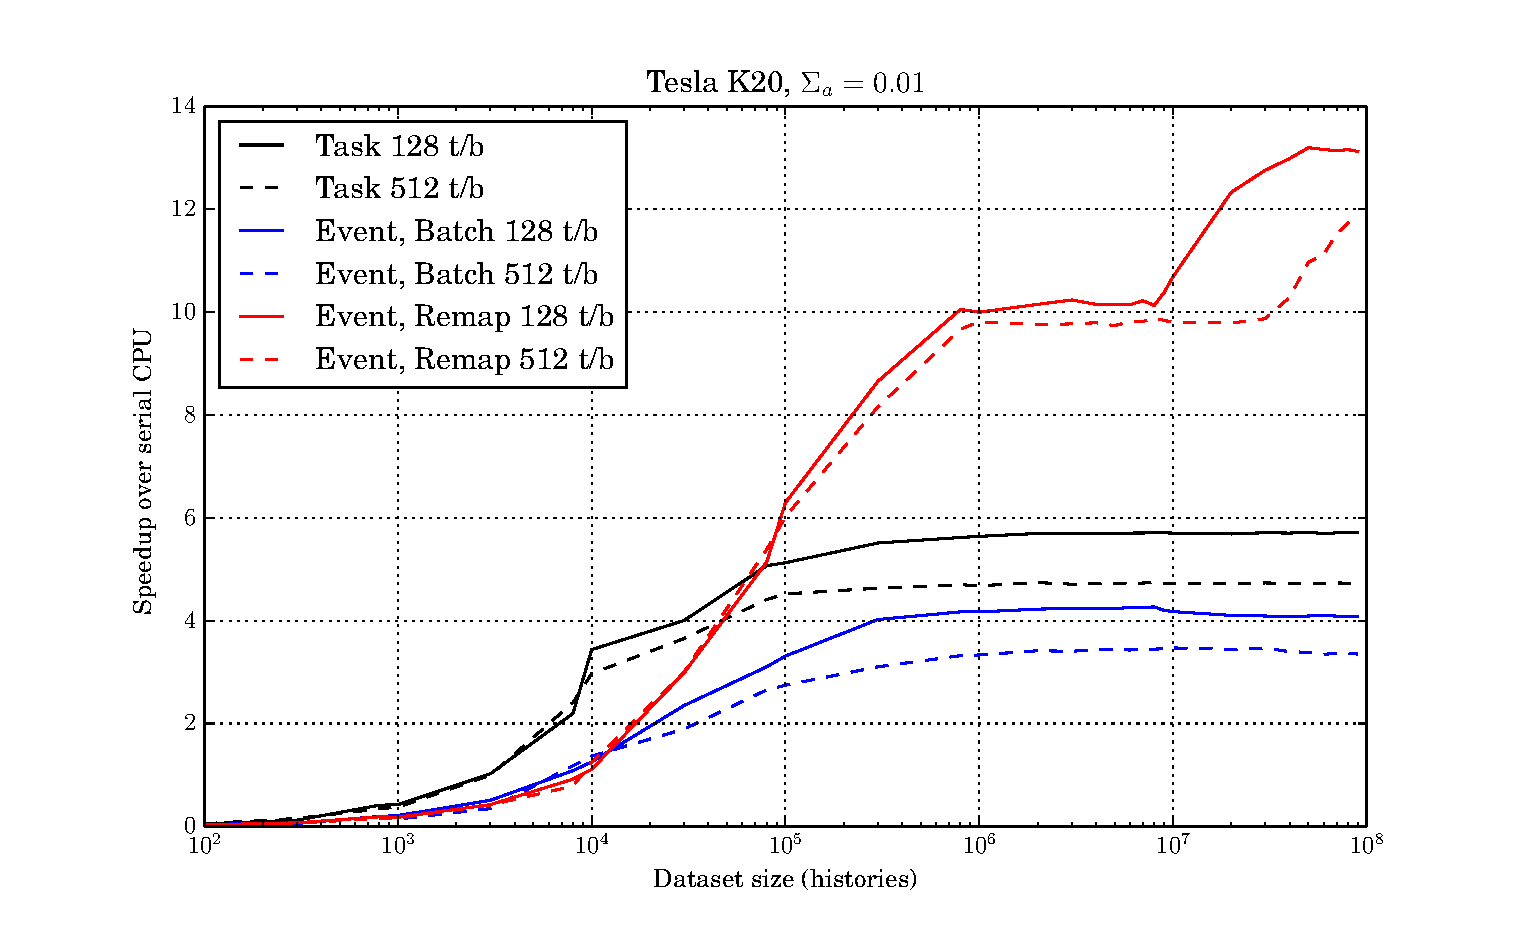
\includegraphics[width=0.8\textwidth]{graphics/prelim_speedup_001_k20.eps}
     \caption{Speedup factors of the GPU implementations over the CPU implementation on a Tesla K20. \label{prelim_speedup_01} }
\end{figure}

\begin{figure}[h!] 
  \centering
    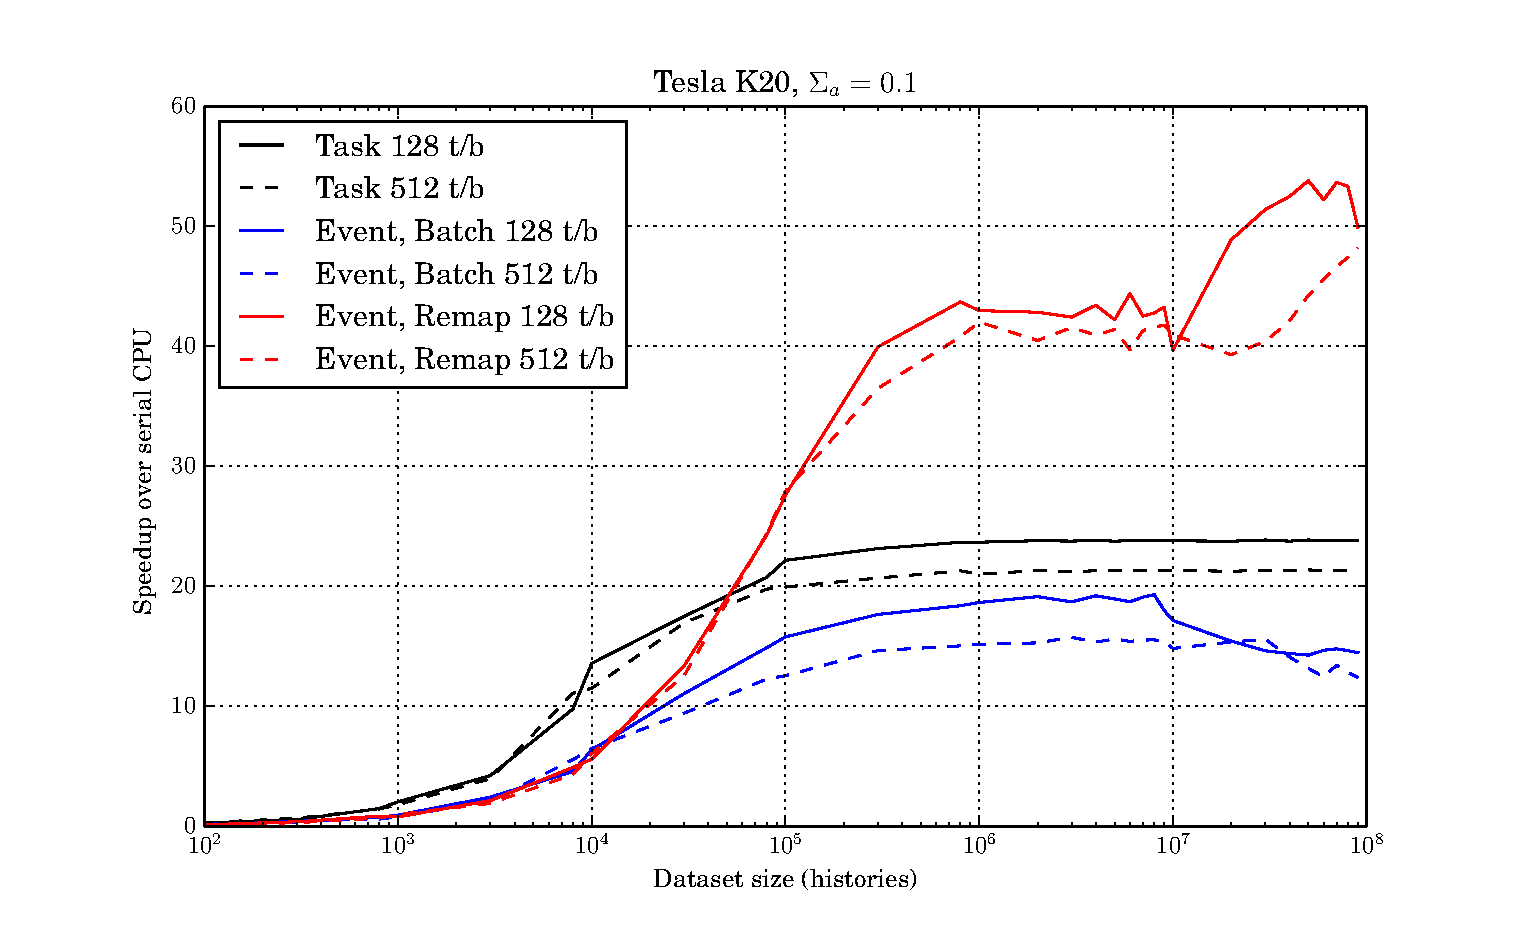
\includegraphics[width=0.8\textwidth]{graphics/prelim_speedup_01_k20.eps}
     \caption{Speedup factors of the GPU implementations over the CPU implementation on a Tesla K20, but with $\Sigma_a$=0.1 in cell 0. \label{prelim_speedup_1} }
\end{figure}

Figure \ref{prelim_active} shows the number of active histories per transport iteration for the batches and remapping implementations.  Since the remapping implementation eliminates all references to terminated particles, the data loaded into the threads blocks is all active and no threads return without doing work.  The figure clearly shows that the blocks are kept full until the end of the simulation when the remain number of particles becomes less than the maximum number of threads.  It also shows how quickly particles are depleted from the blocks.  In this simple case, most interactions happen in cell 0 by far, and particles are absorbed almost identically to \eqref{depleted}, where $i$ is the iteration number and $\Sigma_a/\Sigma_t$ is the absorption probability in cell 0.   Figure \ref{prelim_active} does not reflect the time taken by each iteration, however.  The iterations with more particles take longer than those with fewer for both implementations.  More particles are transported per time in full iterations, however, as evidenced by the greater speedups of the remapping algorithm in Figure \ref{prelim_speedup}.

\begin{equation}
\label{depleted}
\frac{N}{N_0}=\exp \left(-\frac{\Sigma_a}{\Sigma_t} i \right)
\end{equation}

\begin{figure}[h!] 
  \centering
    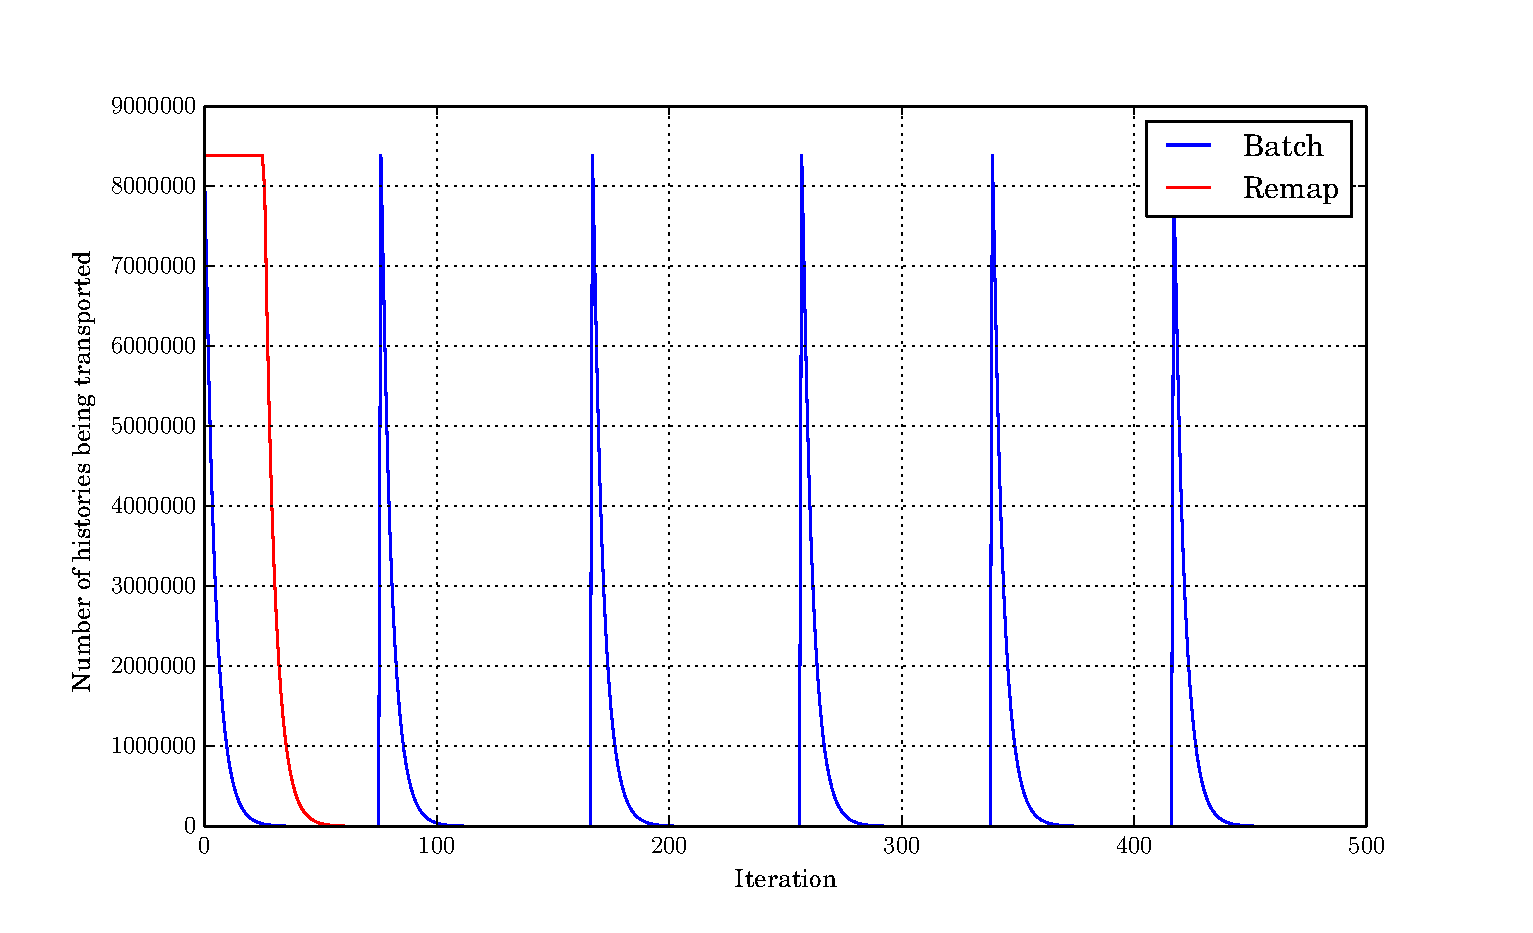
\includegraphics[width=0.8\textwidth]{graphics/prelim_active.eps}
     \caption{The number of actively transporting threads for the event-based GPU implementations. \label{prelim_active} }
\end{figure}

The most likely reasons that the task-based implementation outperforms the event-based is due the simplicity of the problem and the communication and setup overhead associated with many kernels being launched from the host.  Since the problem is so simple, all the data fits into local memory and the latencies associated with accessing global memory often are hidden.  The purpose of this study was to eliminate memory transaction and only focus on thread divergence, but memory transactions will have a very large impact when real cross sections and geometries are used.  Also only having two reactions means threads only diverge when they terminate.  WARP will have many reactions types to deal with, and divergence will be a greater problem.  This also allows threads in a block to almost always be in the same step of the transport algorithm, further eliminating divergence implicitly.  Despite this, the study does show that control flow divergence is greatly reduced by using an event-based algorithm, as shown by Figure \ref{prelim_divergence}.  The overhead of calling kernels many times in the event-based implementations is most likely the reason for the poorer performances.  It should also be noted that compiling the tests with compute capacity 2.0 (-arch sm\_20 compiler flag) improved performance about 20\% over compiling with compute capacity 3.0.

\begin{figure}[h!] 
  \centering
    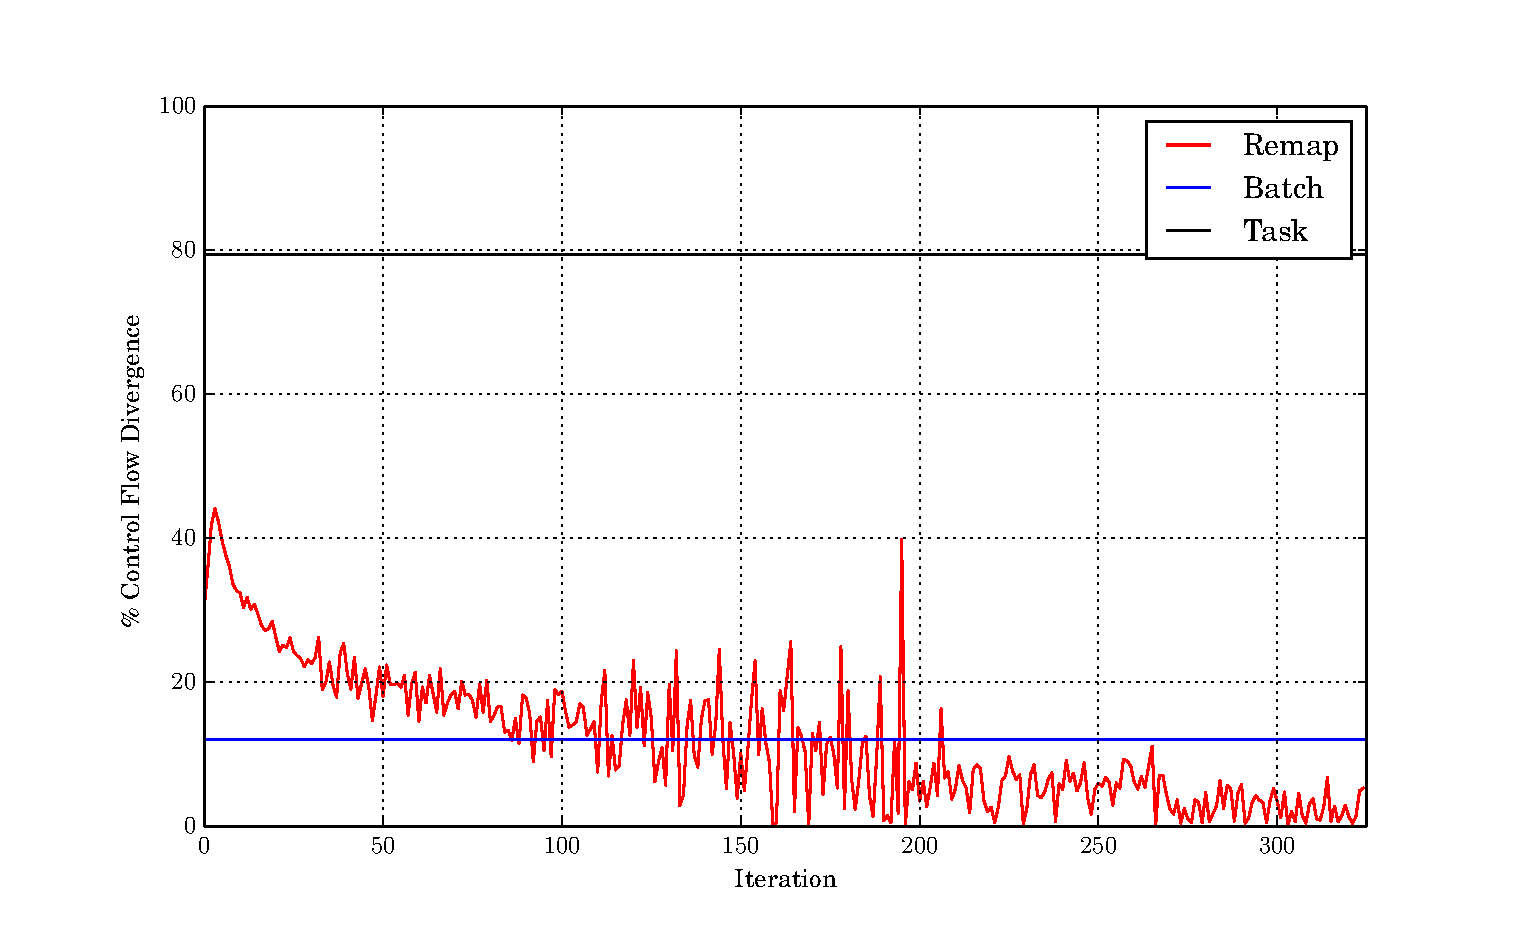
\includegraphics[width=0.8\textwidth]{graphics/prelim_divergence.eps}
     \caption{The \% of control flow divergence of the task- and event-based GPU implementations (UPDATE). \label{prelim_divergence} }
\end{figure}

Another consideration pointed out by this study is that library use and the task-based algorithm are incompatible.  Libraries currently available for the GPU carry out a single task on a dataset, they are not coded for single-thread operation and must be launched as their own kernels.  Having threads in different states wouldn't allow the library routines to be dropped in and carried out consistently across all the active particle data.  Also, much of the performance from optimized algorithms comes from thread blocks cooperating, and using a task-based algorithm would be like treating each SM as a separate CPU (using a stack-popping method) and would minimize the benefits of divide-and-conquer algorithms.

From this preliminary 2D mono-energetic scattering study, it can be concluded that using an event-based algorithm with a compaction/sort algorithm to eliminate terminated particles from being accessed by thread blocks drastically reduces control flow divergence and keeps warps coherent.  There is a cost for adopting this algorithm, however, namely the overhead of kernel launches.  How these factors compete in WARP will be shown in the results in Chapter \ref{chap:results}.  WARP will adopt the event-based algorithm in hopes that thread coherency and its benefits (maximal load coalescing, little warp serialization) will outweigh launch overhead in when real data is used, as well as to allow library usage in complicated parallel tasks.

\subsection{Ray Tracing with OptiX}

Another preliminary study was preformed in order to determine the performance of OptiX when ray tracing from randomized points as well as to find the optimal OptiX configuration for WARP.  In rendering, rays are initialized in a uniform array, but the flexibility from writing custom ray generation program in OptiX allows for arbitrary starting points and directions to be used.

\subsubsection{Point-in-Polygon / Material Query}

\begin{figure}[h!] 
  \centering
    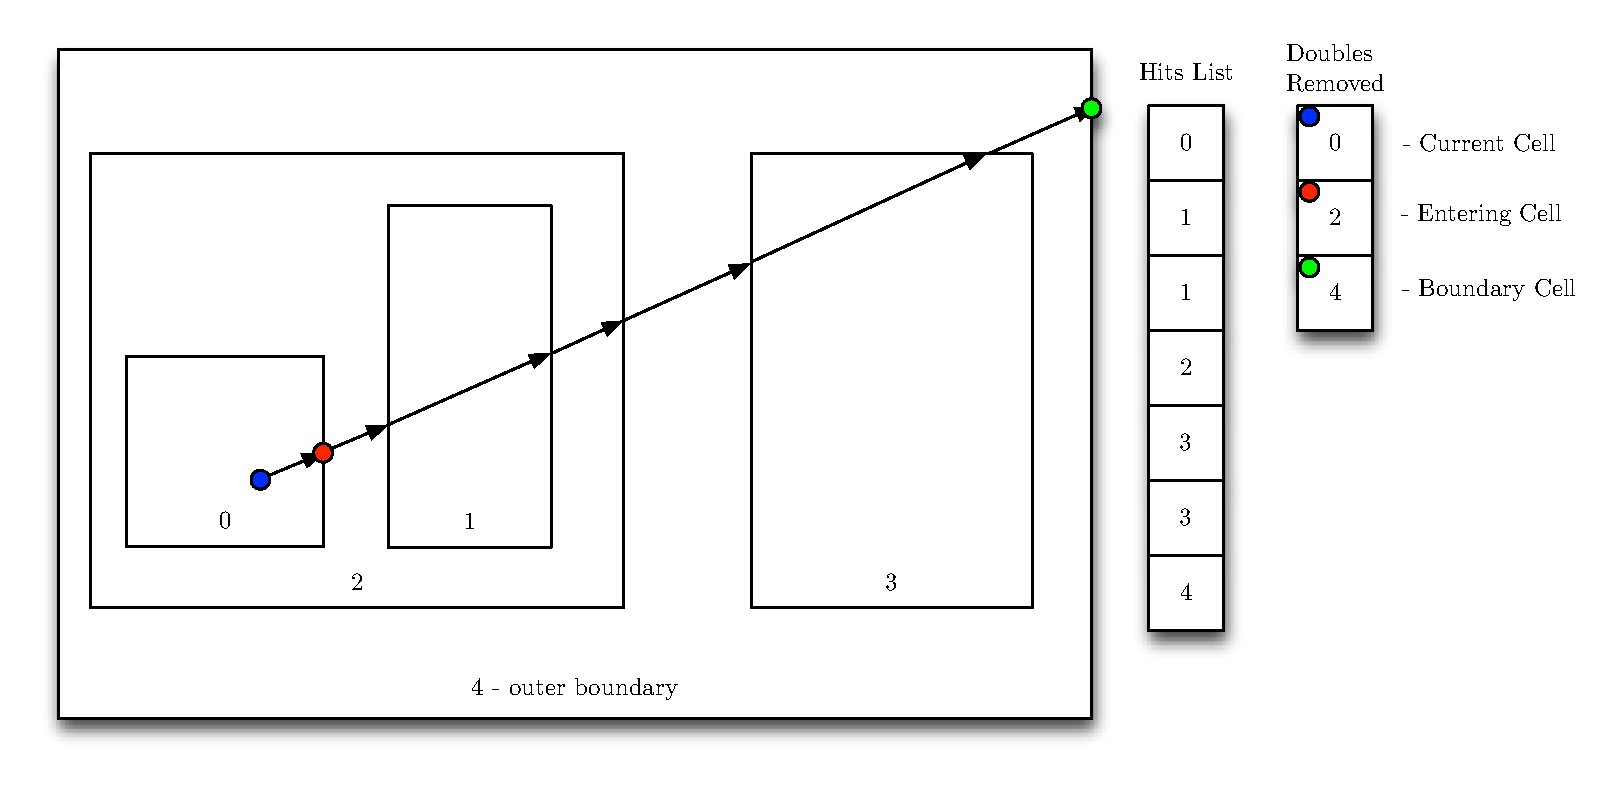
\includegraphics[width=1.0\textwidth]{graphics/whereami.eps}
     \caption{The point-in-polygon-like algorithm for determining the entering cell number by using ray tracing \label{whereami} }
\end{figure}

An important job for the geometry routine in a Monte Carlo neutron transport code is to determine the cell and material IDs of a particle based only on it's coordinates.  This is very important in Woodcock tracking, since surface intersections are not calculated and this material query it is the only place where geometrical information enters into the simulation.  In WARP and other ray-tracing codes, material information is only updated when a neutron sampled interaction distance is greater than the near surface distance.  In this situation, the neutron is placed on the boundary, the material information is updated for the new material, and the interaction distance is sampled again using the same direction of flight as before.  WARP will use and algorithm to determine the entering cell number by using ray tracing, since all the geometrical information is stored in the OptiX context.  This will also mean the material query will be able to take advantage of the OptiX acceleration structures, and should scale well (logarithmic).

The material query algorithm is shown in Figure \ref{whereami}.  An ordered list of surface intersections is generated by iteratively ray tracing and adding the closest surface number to the hit list.  Tracing is terminated when a predefined outer cell is intersected which all other cells are inside of.  Since all surfaces are closed, the ray will intersect any cell surface twice that it isn't nested in.  When the list is made, the double entries are removed, which yields a list of cells the neutron is nested in.  The first entry will be its current cell and the second entry will be the cell it is entering into.  It is important to make the scene epsilon an appropriate value for the geometry if this algorithm is to be used effectively.  The scene epsilon determines the minimum intersection distance possible, i.e. the distance away from the source point which intersections are allowed to occur.  This prevents self-intersections from happening due to numerical inaccuracies.  The mathematical cell descriptions are exact, but the number representing them are not, and if they are treated as exact, a situation can occur where a neutron is placed at a boundary, but it is actually slightly behind the boundary due to floating-point roundoff.  When the next trace is started, the ray intersects the boundary it has already intersected with instead of tracing into the next cell.  Giving OptiX a scene epsilon guarantees the trace starts after the very near boundary, and accurate results are calculated.

This algorithm is very similar to the ray casting point-in-polygon algorithm which determines if a point is inside or outside of an arbitrary polygon by counting the number of times it crosses a surface.  An even number means it is outside and an odd number means it is inside.  This algorithm is almost the same, but it keeps track of cell numbers instead of binary logic for one surface.  This way, the nesting of a neutron can a be determined and the entering cell can be found.  Both of these algorithms take advantage of the cell being closed, and in this sense is similar to Gauss's Law or the divergence theorem which states the flux integrated around a surface will be nonzero only if the surface contains a source.  This material query algorithm is like a discrete, single field line version where the neutron's position is the source point and the cell boundaries are the integrating surfaces.

An important consideration in this type of geometrical representation is that the volume of a cell is \emph{always} the spatial intersection of the space inside of the cell with space outside any cells nested inside it.  For example, if two cube cells were specified to be centered at the origin with cube 2 completely encompassed by cube 1, the space in-between cube 1 and cube 2 would belong to cell 1 while the space inside cube 2 would all belong to cube 2.

\subsubsection{Instancing}

\begin{figure}[h!] 
  \centering
    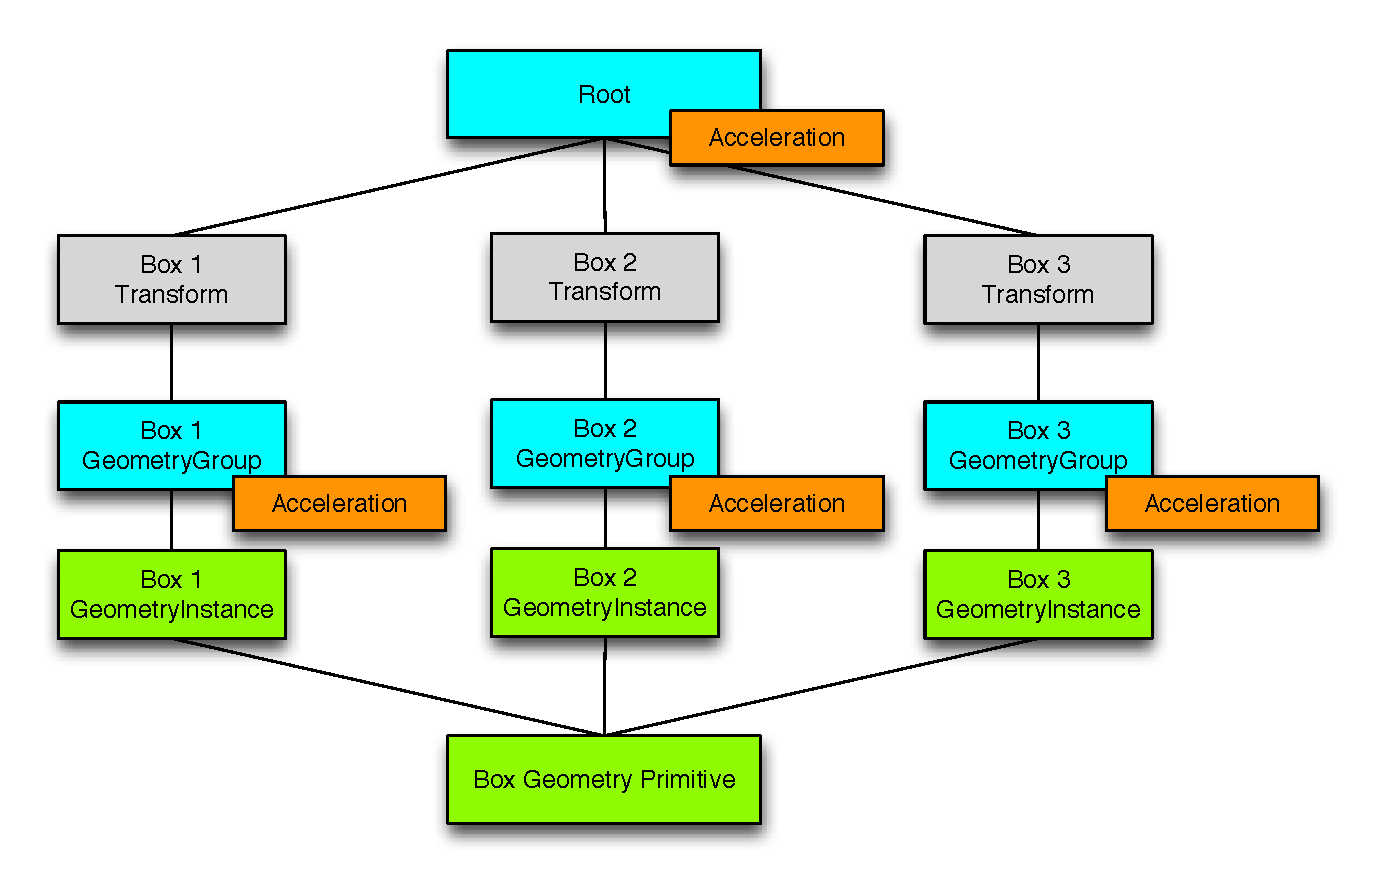
\includegraphics[width=0.8\textwidth]{graphics/transform_instancing.eps}
     \caption{The OptiX node graph using transform instancing \label{transform_instancing} }
\end{figure}

Nuclear reactors can have very complicated geometries, but they basically rely a simple shapes that are repeated in arrays.  There are a few ways in which identical cells can be instanced in OptiX.  the first and most convenient is to define a single primitive in it's own coordinate system, then use a transform node (shown in Figure \ref{node_graph}) in the OptiX node graph to transform the primitive to it's actual position via an affine transformation matrix.  The resulting node graph is shown in Figure \ref{transform_instancing} for a scene that has three boxes in it.  As a reminder, a GeometryInstance objects ties a hit program to the spatial geometry data in the geometry primitive object, acceleration objects are attached to all group objects, and transform objects can only have children that are Group or GeometryGroup objects which is why each GeometryInstance must have its own GeometryGroup.

Transform instancing is convenient since only a single primitive needs to be defined.  If another instance is needed, one can simply apply a transform matrix to it and all the work is done by OptiX.  This scheme has a lot of overhead, however, since each instance has it's own group and its own acceleration object, producing a deeper node graph than necessary.

\begin{figure}[h!] 
  \centering
    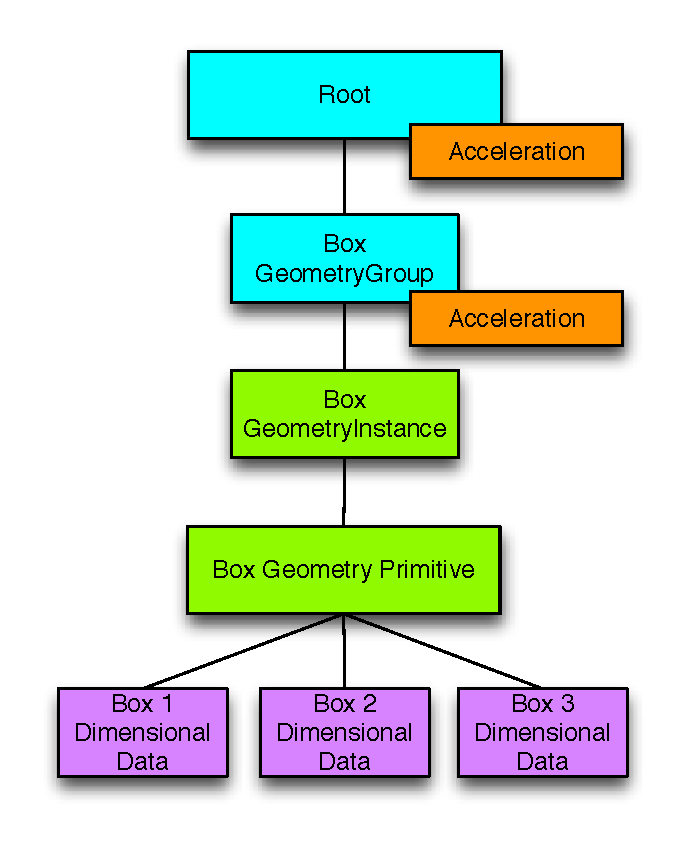
\includegraphics[width=0.4\textwidth]{graphics/primitive_instancing.eps}
     \caption{The OptiX node graph using mesh primitive instancing. \label{primitive_instancing} }
\end{figure}

An alternative instancing method is using mesh-based primitives.  In this scheme, is still a single geometry primitive, but now the primitive is attached to an array of spatial data (and OptiX buffer) that contains the dimensions of each individual primitive.  The transform node no is longer used, since it would transform the whole group instead of a single primitive.   The transforms must be applied to the data beforehand and written into the buffer as separate primitives.  This method produces a shallower node graph with only two acceleration objects and a single GeometryGroup for \emph{all boxes}.  These numbers would not change even if there where 200 boxes in the scene, only the number of data elements on the very bottom of the graph would change.  This is called mesh instancing since the data structure was envisioned for the many triangular surfaces in meshes of complex objects rather than for individual instancing of separate, simple objects.

One goal of this study is to determine which of these instancing methods has better performance and will ultimately be used in WARP.

\subsubsection{Test Geometries}

Three different geometries were used in the test - an assembly-like hexagonal array of cylinders, an assembly of the same size, but with two interleaved arrays, and a much larger version of the assembly-like geometry. These cases were chosen to highlight the scaling and to see the performance of the instancing schemes in common nuclear reactor like scenarios.  Figure \ref{raster_images} shows the geometry for the interleaved assembly and the large assembly.  These figures were created by OptiX by performing a cell number query as prescribed in the previous section.  The interleaved assembly consists of three hexagonal arrays, two on cylinders, and one of hexagonal prisms.  The arrays are 7 elements on a side, which corresponds to 127 elements each for a total of 383 elements (including the large hex cell around the arrays and the outer box cell).  The large assembly has 25 cylinders on a side, for a total of 1803 elements.  The smaller assembly is 15 cylinders on a side, for a total of 633 elements.

\begin{figure}[h!]
\centering
\begin{subfigure}{.5\textwidth}
  \centering
  \includegraphics[width=.9\linewidth]{graphics/prelim/interleaved_assembly.png}
  \caption{The interleaved assembly}
  \label{fig:sub1}
\end{subfigure}%
\begin{subfigure}{.5\textwidth}
  \centering
  \includegraphics[width=.9\linewidth]{graphics/prelim/large_assembly.png}
  \caption{The large assembly}
  \label{fig:sub2}
\end{subfigure}
\caption{Raster images of $x$-$y$ cross sections of the geometry created by using the PIP cell/material query algorithm \label{raster_images}}
\label{fig:test}
\end{figure}

The cell numbers are mapped to colors in the image, and since there are no errors, it appears the routine is working and the algorithm can calculate the cell numbers.  A nice feature of OptiX is that variables can be attached to each geometry primitive.  In addition to the cell ID number, the materiel ID is also attached, so the material query can be done directly by OptiX rather than determining the cell number, then having to do an additional lookup or hash afterwards.

\subsubsection{Results}

Figure \ref{prelim_optix_k20} shows the ray trace rates for running these geometries on a NVIDIA Tesla K20 card.  There are cases for each geometry (assembly, large, and interleaved), whether the trace uses primitive or transform instancing (prim or xfrm), and whether it uses a split bounding volume hierarchy or regular bounding volume hierarchy (Sbvh or Bvh).  These traces all employed the cell number query PIP algorithm, so these rates are representative of the actual rates in a Monte Carlo Simulation where not only the first intersection must be found.  The source point distribution in all cases is uniformly random over all space and isotropically random in angle.  The trace rates are fairly constant after $10^6$ particles, but primitive instancing is always faster than transform instancing, and using BVH acceleration is always faster than SBVH.   The only time this isn't the case is for the interleaved assembly, where transform instancing performs slightly better than primitive instancing.  K-d trees are not used since they require a mesh vertex buffer be provided by the user, which implies that they only work for triangularly-meshed objects, not ones instanced by simple geometric primitives like spheres and cubes.  Handling geometries that are meshed in such a way may be a future area of development in WARP.

\begin{figure}[h!] 
  \centering
    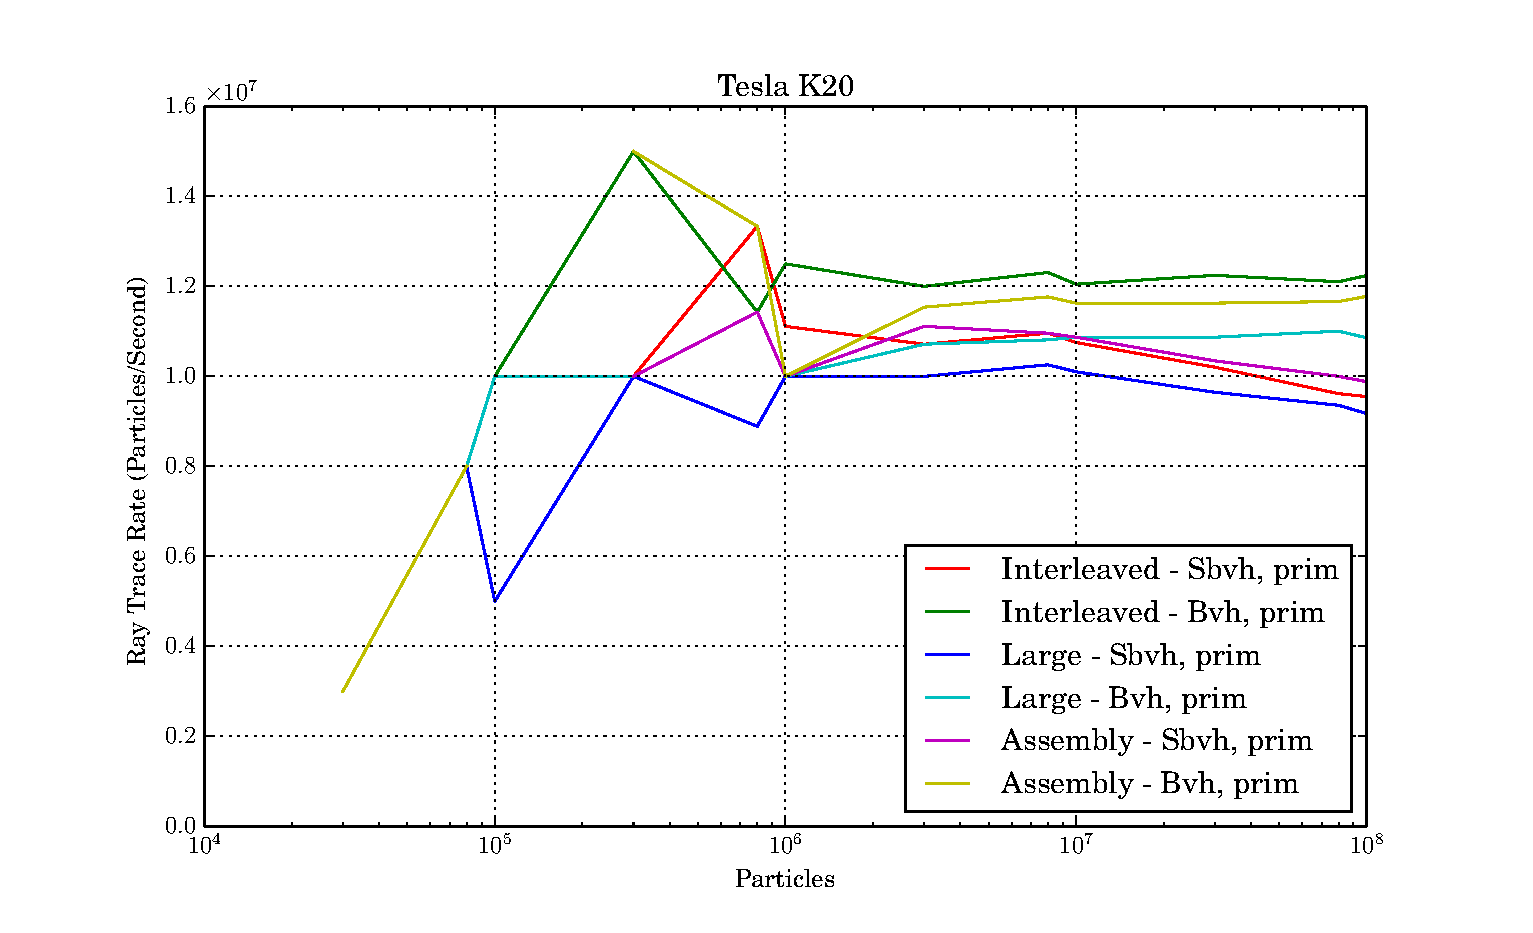
\includegraphics[width=0.8\textwidth]{graphics/prelim_optix_k20.eps}
     \caption{Trace rates of a NVIDIA Tesla K20 performing cell queries with the PIP algorithm. \label{prelim_optix_k20} }
\end{figure}

The interleaved assembly is also the geometry with the least amount of objects.  Another study was done to show the scaling of the two instancing types.  In these traces, a cell query was again done from a uniformly random and isotropic distribution of source points.  The number of source points was set to $8\times10^7$ for every trace in order to ensure being on the trace rate plateau shown in in Figure \ref{prelim_optix_k20}.  A BVH acceleration structure was also used, since this structure showed the best performance.  The geometry used was another hexagonal lattice of cylinders, identical to the assembly and large assemblies test geometries, only with more elements.  The volume, pitch to diameter ratio, and aspect ratios of the large cells were kept constant, but the cylinder radii were halved while doubling the number of elements on a edge.  Figure \ref{prelim_optix_scaling} shows the results of the scaling test, and it can be seen that the ray trace rates for both primitive and transform instancing plateau after about $10^3$ objects in the scene.  Primitive instancing still outperforms transform instancing, especially at very large numbers of objects.  It should be noted that the trace rates for the two dataset sizes start quite different for one object, then converge to equal performance at large object numbers, where the trace becomes more dependent on acceleration traversal rather than output buffer access (where smaller size makes a difference when there are few objects).  Traces were also done in a cell containing no objects, and rates were on the order of ten times faster, which is apparent in the scaling figure.

\begin{figure}[h!] 
  \centering
    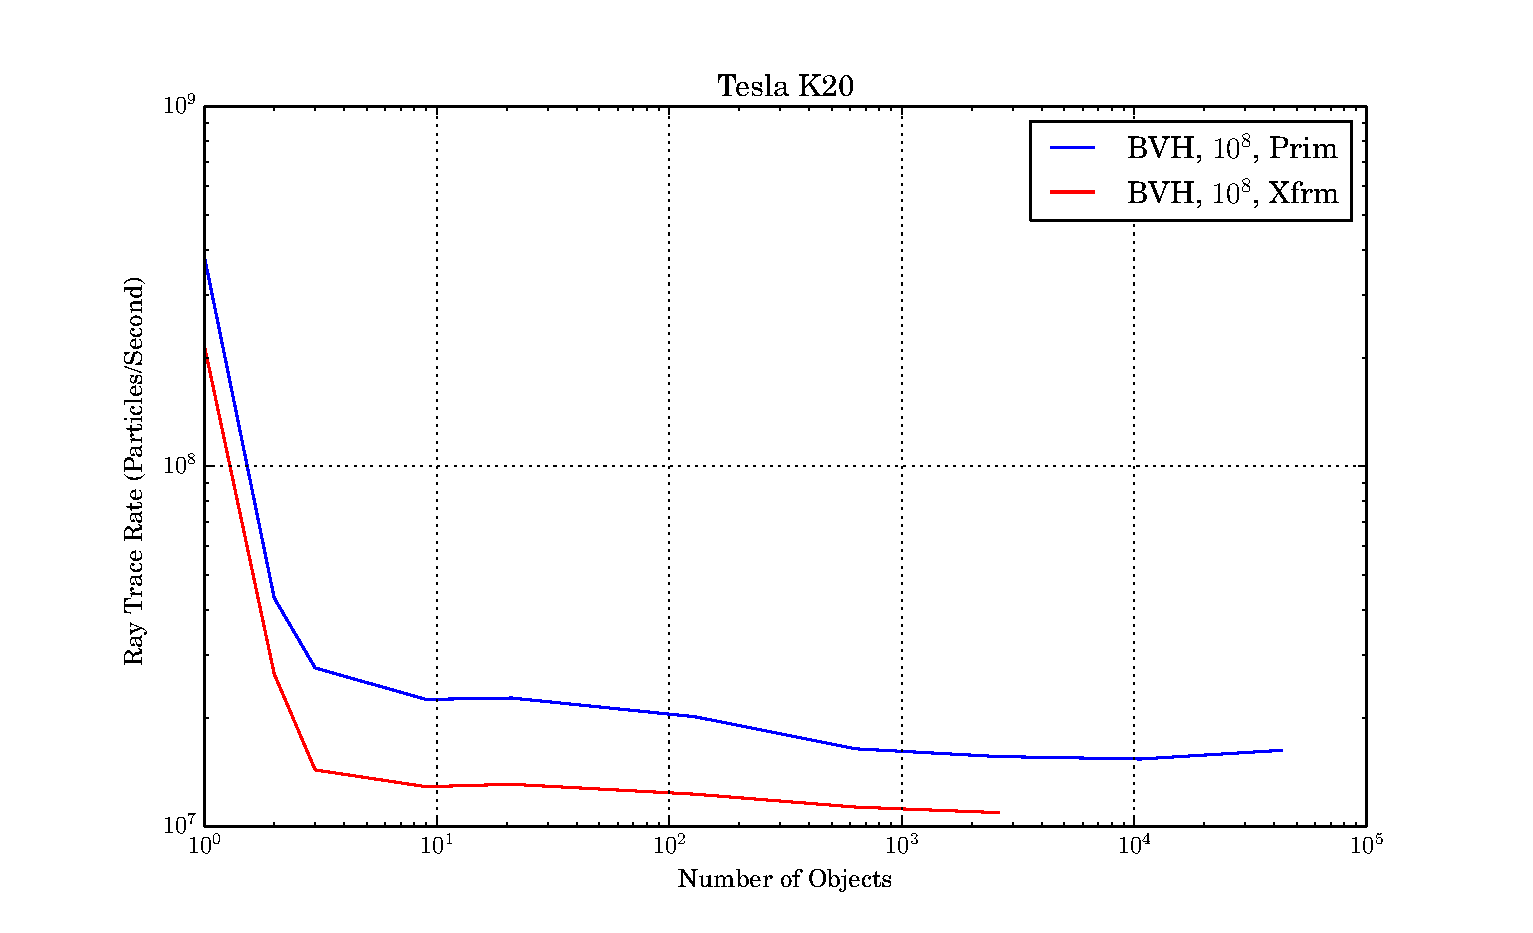
\includegraphics[width=0.8\textwidth]{graphics/prelim_optix_scaling.eps}
     \caption{Trace rate scaling on a NVIDIA Tesla K20 performing cell queries with the PIP algorithm. \label{prelim_optix_scaling} }
\end{figure}

\begin{figure}[h!] 
  \centering
    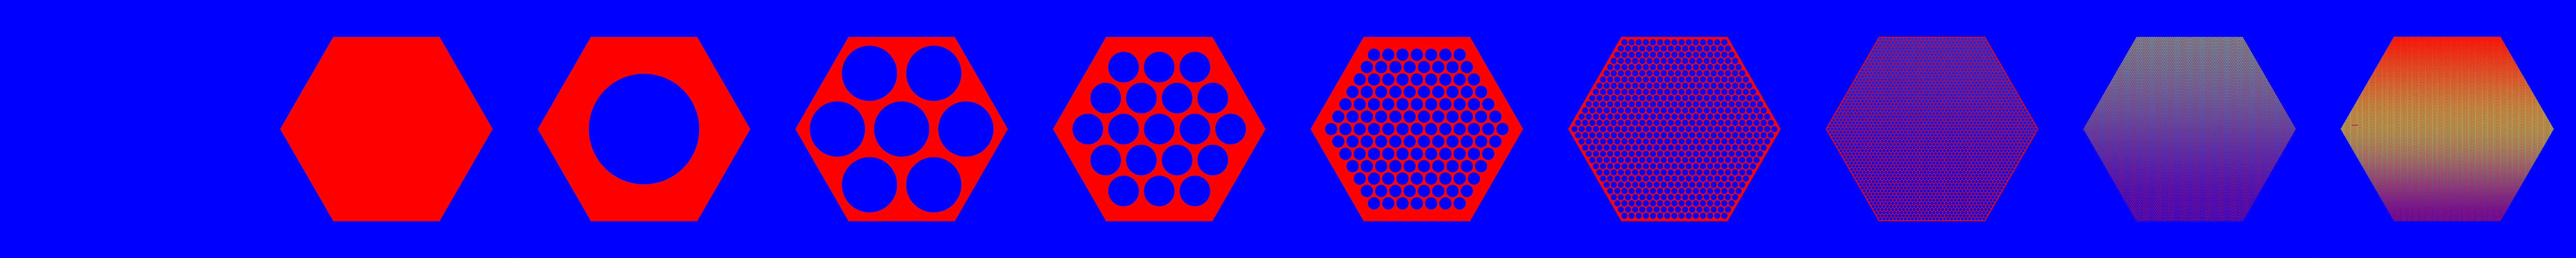
\includegraphics[width=1.0\textwidth]{graphics/prelim/prelim_scaling_geom.png}
     \caption{The geometries used in the scaling study from least number of objects on the left to most on the right. \label{prelim_scaling_geom} }
\end{figure}

Using transform instancing did not work for cell numbers somewhere between 2613 and 10623 cells for the $10^8$ dataset size, and is why transform instancing trace stops at 2613 cells in Figure \ref{prelim_optix_scaling}.   Host memory consumption became too great and the process would be terminated.  Structure construction prior to the trace also became very slow compared to primitive instancing, presumably due to the independent acceleration objects attached to every instance and the overhead of computing all the affine transformations at acceleration structure build time.

Also, traces were done where the direction of every particle was in the negative $z$ direction, since this is the direction with the fewest number of surfaces between the source particles and the boundary cell.  Performance was increased marginally, but this can only be taken advantage in geometries where there is a direction of least heterogeneity (like 2D lattices).

Figure \ref{prelim_optix_G650M} shows the trace rate versus dataset size benchmark, but run on a NVIDIA GeForce GT 650M, the discrete graphics card in a MacBook Pro, Mid-2012 Retina model.  The same trends can be observed, except that overall trace rate is much slower, which is not surprising, and that the impact of transform instancing is very pronounced in runs with fewer particles.  This study was done to simply show the performance of a smaller, non-compute card compared to that of the Tesla card.

\begin{figure}[h!] 
  \centering
    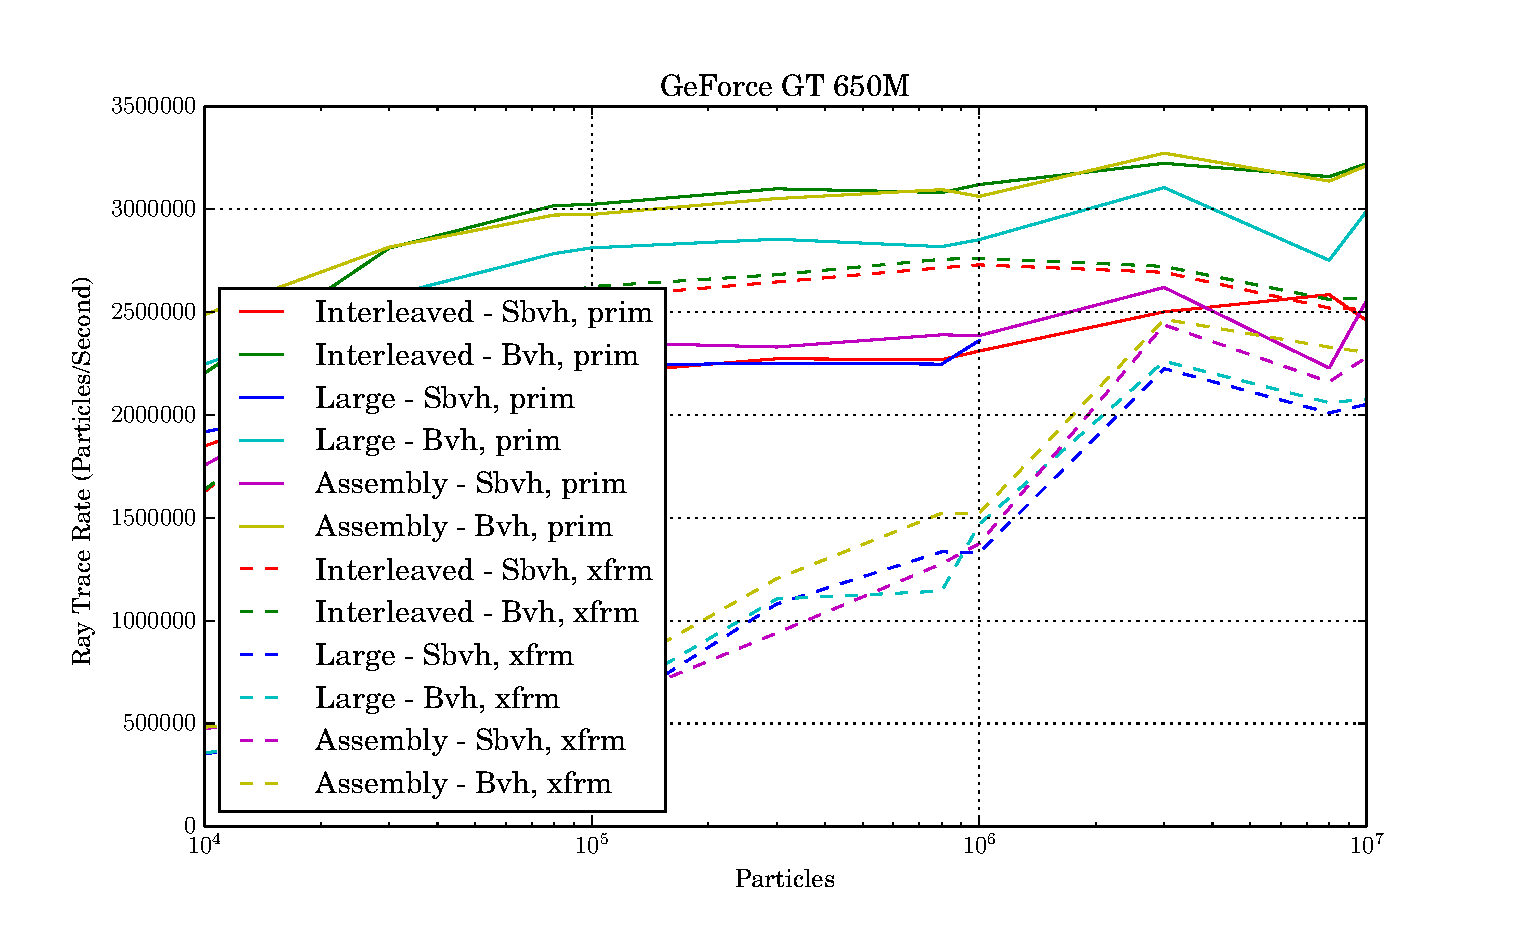
\includegraphics[width=0.8\textwidth]{graphics/prelim_optix_G650M.eps}
     \caption{Trace rates of a NVIDIA GeForce GT 650M performing cell queries with the PIP algorithm. \label{prelim_optix_G650M} }
\end{figure}

From these preliminary results, it can be concluded that XXX.


%%%%%%%%%%%%%%%%%%%%%%%%%%%%%%

\section{WARP in Detail}

The preliminary studies show that thread divergence can be effectively reduce with CUDPP without incurring huge costs, large datasets need to be run in order to hide memory latency, and a BVH acceleration structure in OptiX performs best for randomly-oriented distributions of rays.  Since most data will be access randomly no matter what, the layout will be regularized as much as possible and the particles will be sorted by reaction, sweeping out completed particles and grouping similarly-interacting particles together to maximize warp coherence and occupancy.  Since histories complete randomly, history data access will become sparse even if sweeping out is not done, and the radix sort will preserve monotonically increasing thread IDs within a reaction group, so it's impact on data access should be small, and the only cost be that of performing the operation.

As stated before, WARP will read ACE-formatted data, perform all reaction types as prescribed by them, use a Serpent-like unionized energy grid to regularize data access, use an event-based transport algorithm with parallelized operations for sorts and sums, use OptiX for general 3D geometry representation (without explicit nesting), use a SOA for neutron history data, and perform all operations on the GPU unless strictly forbidden.  From here on, it will be expanding the preliminary studies.  OptiX will be used for 3D geometry representation, physics routines that use real cross section data will be made in CUDA, the compaction routine in CUDPP will be substituted for a radix sort, tallies will be implemented, as will criticality and fixed source methods.  These expansion will yield WARP, a program for continuous energy Monte Carlo neutron transport on GPUs in general 3D geometries, which will be compared for accuracy and execution speed against Serpent and MCNP.

WARP will be written in C/C++ with some Python (which will be explained later in this section), and will rely on the OptiX framework for geometry representation and the CUDPP libraries for dataset-wide parallel operations. Single precision floating point number will be sued throughout in order to realize the full computational capacity of the GPU and to allow simulations to be carried out on more affordable and higher clocked GeForce cards.  Double precision is only needed XXX \cite{please}.

At this point, all the geometry routines are have been described in detail and the subsequent sections will discuss the cross section data access patterns and the energy related routines.

%%%%%%%%%%%%%%%%%%%%%%%%%%%%%%

\section{Data Layout}

As described in Chapter \ref{chap:background}, the nuclear data required in Monte Carlo simulations is very heterogeneous.

\subsection{Unionized Cross Sections}

It is particularly troublesome that each cross section has its own independent energy grid.  Using point-wise data for continuous energy simulations requires an interpolation be performed between points, and to do this, the code must somehow scan the energy grid array to find the points between which the neutron's energy falls.  If every isotope has its own grid, this search must be done for every isotope, and can become very expensive.  This is why the unionized energy grid structure, like that implemented in Serpent, is used by WARP \cite{jaakko_xs}.

Unionizing the cross sections simply means that the energy grids of the cross sections are all unionized into a single, larger vector which every isotope can use, i.e. many 1D vectors and transformed into a single 2D matrix indexed by incoming energy and MT reaction number.  Doing this makes holes the the data, however, but these are filled by linear interpolation.  Since linear interpolation is always used to interpolate the cross sections, no information is lost and the cross sections are preserved.  The resulting dataset is larger than the sum of the individual cross sections, however, since it contains redundant data.  This is the tradeoff between regularizing the data in this way as opposed to accessing the energy grids separately.  The dataset will use more memory, but will be much easier to search.  Figure \ref{unionized_layout} shows the unionization process with two small, arbitrary energy grids and their corresponding cross section vectors.  The colors in the unionized energy grid represent which isotope the grid value came from, the green cross section data blocks are interpolated values, and the red blocks are placeholder zeros to preserve thresholds.

\begin{figure}[h!] 
\centering
\includegraphics[width=0.6\textwidth]{graphics/unionized.eps}
\caption{Unionizing two cross section vectors. \label{unionized_layout} }
\end{figure}

With the cross sections unionized in this way, once the bounding energy indices, $E_i<E<E_{i+1}$ , are found by single search, the cross section values for every isotope can be read along a single row.  This format reduces the number of energy searches needed as well as promotes data locality by keeping all the data points for all isotopes this range adjacent to each other in memory (if row-major matrix format is used).  On CPUs, this can be read as cache line and accessed quickly by the cores.  On a GPU, since a thread needs to read the entire line in sequence in order to compute the macroscopic cross section on-the-fly, the memory loads are no coalesced and memory bandwidth is wasted (adjacent threads do no access adjacent memory at the same time).  How WARP computes the macroscopic cross section is explained later.  To mitigate this inefficiency, the data can be recast to use the  \lstinline{float4} datatype, which is a vector type that is 16 byes long.  When requested, the entire 16 bytes will be loaded in one transaction rather than 4 separate transactions, maximizing bandwidth and minimizing the number of global requests (and reducing the impact of latency).

\subsection{Distribution Data as a Linked List}

The cross section data can be regularized with the above method, but there are other data distributions that WARP needs to conduct accurate simulations.  The most prevalent of which are scattering matrices which give tabulated probability distributions for outgoing CM angle $\mu$ and incident neutron energy.  Since these matrices have their own incoming energy grid these values can be unionized into the cross section dataset as well.  This transforms many 2D scattering matrices into a 3D matrix indexed by incoming energy, outgoing $\mu$, and reaction MT number.  Since the energy grid of the scattering matrices are often much, much coarser than the main cross section energy grid, this operation produces a \emph{very large} amount of redundant data.  It was attempted with uranium-235, and resulted in a 3D matrix that was 6.4GB (30991 energy grid points, 598 $\mu$ CDF points, 51 reactions).  This is just for a single isotope and just for the angular distributions of all reactions, and the dataset already cannot fit on the on-card DRAM on most GPU cards.  

After determining that unionizing with the main energy grid was an unacceptable method, another approach was tested where the energy grids of the scattering matrices were unionized between themselves, but not with the main energy grid.  This would reduce the amount of redundant data, but would require an additional search be made on the unionized scattering matrix energy grid.  The memory usage of this method with uranium-235 was reduced to 12MB (103 energy grid points, 598 $\mu$ CDF points, 51 reactions).  When tested with uranium-235 and -238, usage for the scattering data increased to 68MB (171 energy grid points, 1072 $\mu$ CDF points, 97 reactions).  When tested with uranium-235, uranium-238, oxygen-16, and hydrogen-1, usage became 1.1GB (1325 energy grid points, 1237 $\mu$ CDF points, 170 reactions).  Therefore, this method was also deemed to costly.  The distributions have to be left in their original formats, especially on GPUs where storage space much more limited compared to CPUs.


\begin{figure}[h!] 
\centering
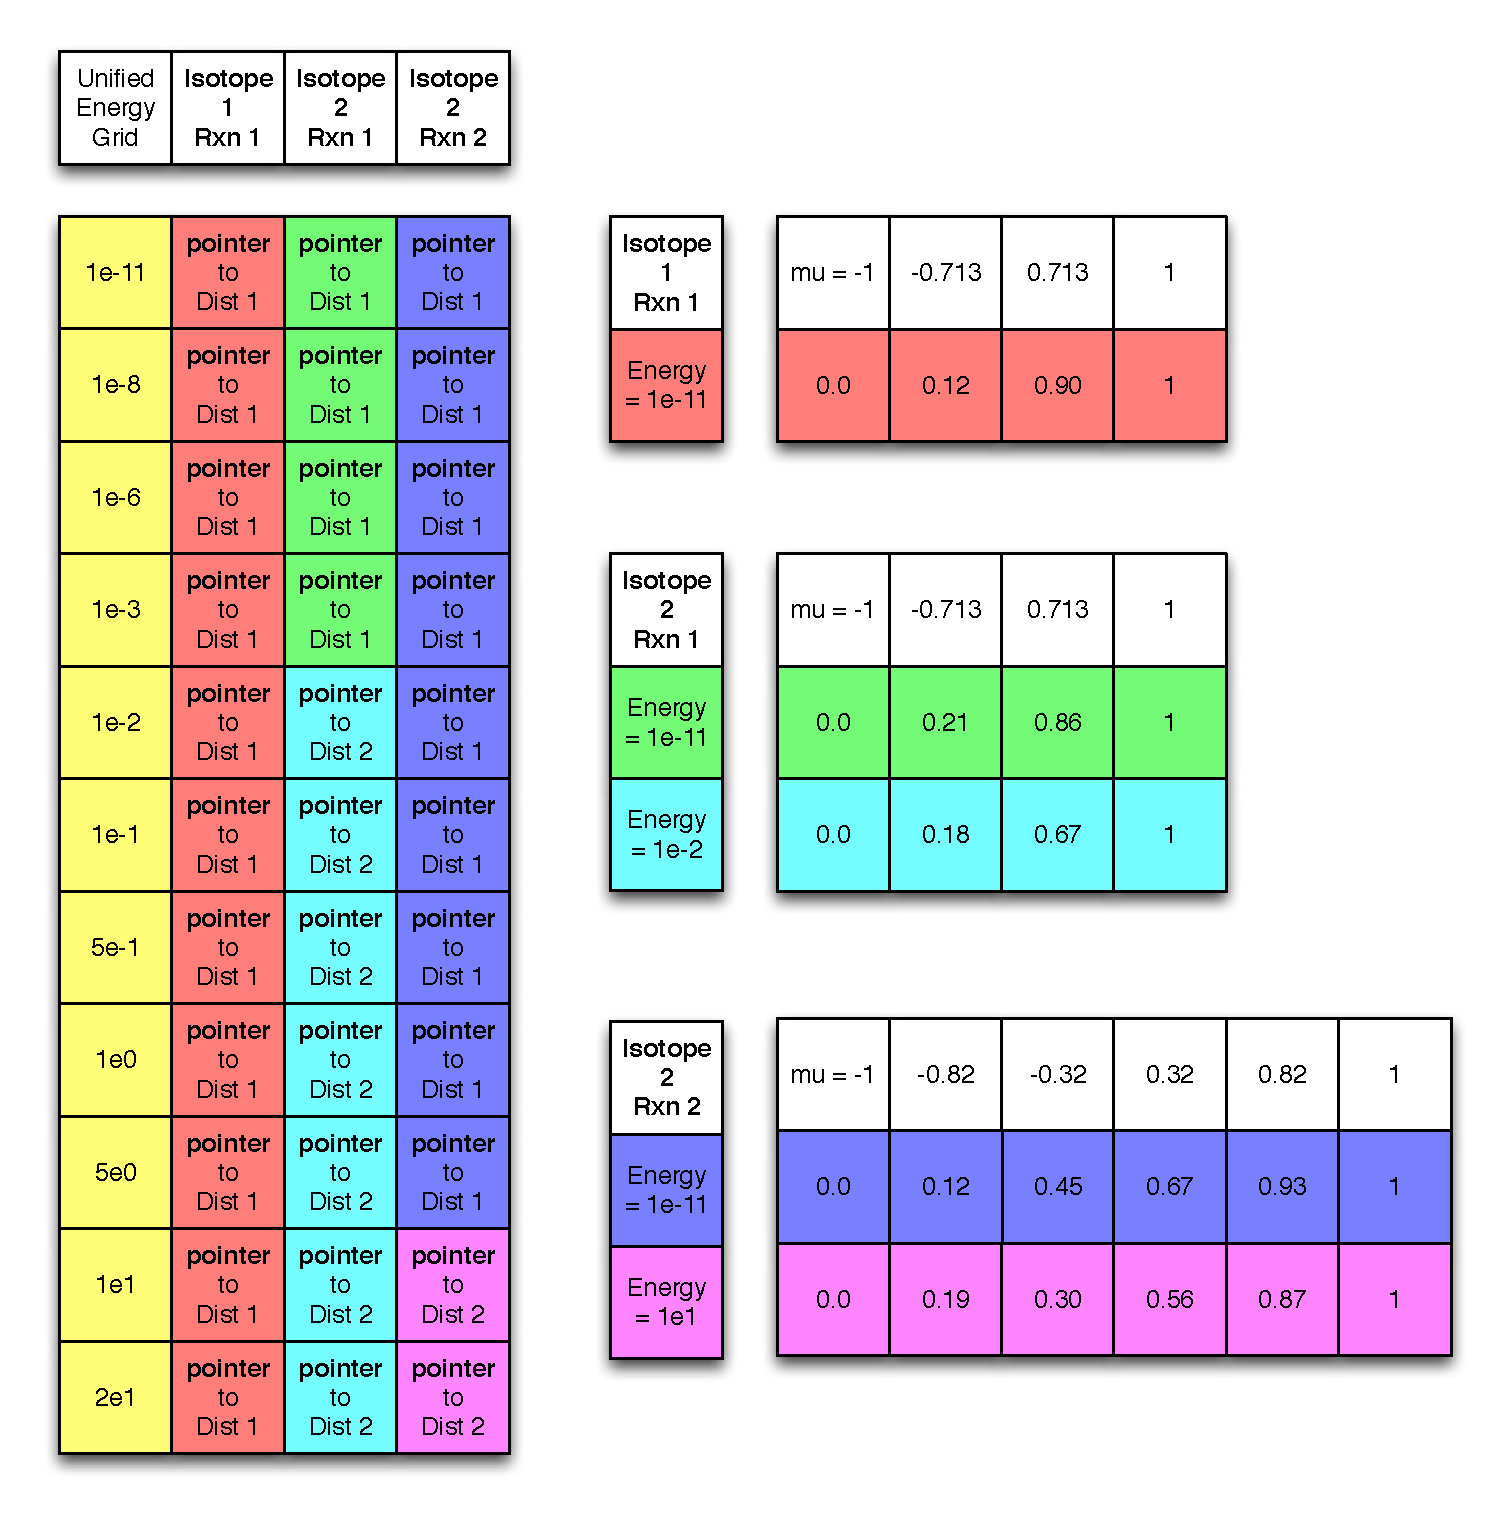
\includegraphics[width=0.7\textwidth]{graphics/unionized_pointers.eps}
\caption{Making a link to distribution data in the unionized dataset. \label{unionized_pointers} }
\end{figure}

After these failed attempts how to resolve the data heterogeneity problem, a method was formulated to eliminate the secondary energy search without having massive data replication.  This method introduces two new matrices identical in size to the unionized cross section matrix, but instead of containing data values, they contain pointers to the location of the appropriate distribution data for the reaction at the energy index determined by the grid search.  Two matrices are needed - one for the scattering distributions and another for the energy distributions.  This way, the unionized dataset is only replicated 3 times, the distribution data can be copied to the card in it's original format, and only a single gird search needs to be performed.  This is similar to a linked list, where a there is a pointer at the end of an object pointing to the next object in a list.  In this case, once a reaction is sampled to occur, there is a pointer readily available at the same index in a second matrix to the appropriate distributions, and no searching needs to be done.  Since the distribution PDFs need to be read serially by each thread, the float4 format can also be of use here.  If there is are distributions for a particular reaction or energy, a null pointer is inserted into the matrix.  For fission reactions which do not have scatting distributions (neutron emission can be assumed to be isotropic \cite{openmc}), the $\nu$ value for the grid energy is stored in the scattering pointer matrix instead of a pointer.  This way a search for the appropriate $\nu$ value does not have to be performed either.  Figure \ref{unionized_pointers} shows a pointer matrix for the unionized cross section matrix in Figure \ref{unionized_layout}.

\subsection{Embedded Python}

The data layout has been described, but not how the data is loaded or reformatted.  An initial effort was made to write a ACE-parsing script in C from scratch, but this was abandoned in favor of using the ACE module of the PyNE package and not reinventing the wheel.  The PyNE (Python for Nuclear Engineering) package ``is a suite of tools to aid in computational nuclear science \& engineering. PyNE seeks to provide native implementations of common nuclear algorithms, as well as Python bindings and I/O support for other industry standard nuclear codes.''  It contains a Python module that can parse ACE data files into python objects which can be more easily handled than flat data arrays.  This module was written by Paul Romano as a preliminary project for OpenMC, whose ACE library was later written in Fortran based on the methods developed in this Python module.  

Some parts of PyNE have a C++ API as well as a Python API, but this is not the case for the ACE module.  It was originally written in Python, not C++, so it has no C++ API.  This created a problem for WARP, since it is written in C/C++, and could not directly make use of the ACE module.  Fortunately, there is a very effective C API for Python!  This API allows one to initialize and run a Python instance from a C program.  In WARP, this API is used to start a python instance where PyNE can be used to load cross sections from ACE data files.  NumPy is then used to unionize the energy grids of the requested isotopes and perform the linear interpolation to fill in the gaps.  Once this is done, the Python instance returns the NumPy array to WARP as a C data structure.  The data is copied to an internal array and the Python object is cleared.  WARP then loops through the unionized array, requesting distribution data from the Python instance.  The scattering and energy distribution data is also copied for the requested energy range in a similar fashion, and a device pointer for the distribution is written into the scattering and energy pointer matrices.  When all the needed data has been copied over to WARP, the Python instance is terminated and its memory freed.  Since the unionized energy grid is an index of the matrix that needs to be searched before a row of the unionized cross section matrix can be accessed, it is stored as its own contiguous array rather than a column of the matrix.  Figures \ref{unionized_layout} and \ref{unionized_pointers} show it as a column simply for illustrative purposes.

The unionized cross section dataset in WARP is resident in the global memory of the GPU.  Storing it in constant memory would seem to make sense, but since it is limited to 64kB, the entire dataset simply cannot be stored here.  Texture memory was also considered, as this could possibly contain all the data, but it is optimized for 2D data locality, whereas the dataset format is mostly access linear fashion across rows and randomly across columns (since energy-changing reactions are sampled randomly).  Both the constant and texture memory spaces are cached, so the inescapable  random access inherent in Monte Carlo simulations may make cached access worse than non-cached due to cache miss penalties.  This effect was not studied in the initial development of WARP, however.  Nelson reports using the constant memory space in his simulations, with little to no performance improvement \cite{nelson}.  Using the texture memory to store the cross section matrix might benefit from the free linear interpolation that can be performed with the texture element load, however.

In its current state, WARP does not use the thermal scattering (S($\alpha,$$\beta$)) tables or unresolved resonance parameters.   These tables improve the physical fidelity of the simulation, but these features can be turned off in production codes and direct comparisons ca be made without them.  Their incorporation may lead to more divergent program flow, but this is left as a area of future work.

\subsection{Python Wrapper}

Work is also underway for wrapping the WARP shared library with Python.  This would be done via SWIG, a piece of software that automatically wraps compiled languages like C/C++ in high-level scripting languages.  This is being done for convenience and usability reasons.  With the C++ classes exposed in Python, the main() function can be replaced with a Python script, eliminating the need to recompile WARP applications when different geometries or run parameters are desired.  This also deviates from the standard flat text input file structure that most Monte Carlo codes use.  Flat text input relies on keywords and adds a layer where input files need to be parsed and data structures built in the application from the information parsed from them.  Using Python to directly access the classes and their data removes this layer, and allows a user to build complex applications.  Since the results would also be resident in a Python session, they would be easily available to the user in their native format for potting scripts or analysis tools.  In text file based output, this information needs to be parsed out with a user written function or done by hand, leading to areas where human error can enter the analysis.

%%%%%%%%%%%%%%%%%%%%%%%%%%%%%%

\section{Tasks}

Now that the necessary data has been loaded and reformatted in a GPU-friendly way, the details on the actual process of transporting neutrons will be described in this section.  Neutron transport consists of an inner and outer transport loop.  The inner loop, shown in Figure \ref{warp_inner_loop}, actually transports the neutrons through the problem geometry and samples the reaction CDFs.  The blocks in the figure represent independent kernel launches, and are executed left-to-right.  The first step is using OptiX to perform the material query, since this information is needed to query the proper cross sections, and to determine the distance to the nearest surface along the neutron's path of travel.  Once this is known, a kernel is launched to do a search on the unionized energy grid to determine the index $i$ which satisfies $E_i<E<E_{i+1}$.  From here the macroscopic kernel is launched which computes the total macroscopic cross section for the material, samples the interaction distance, which isotope the neutron interacts with, moves the neutron to the nearer of the interaction/intersection distance, and sets the neutrons reaction number to the resample flag if the intersection is closer.  Since the macroscopic cross section has been computed, the tally kernel is launched which scores a specified flux tally.  After the flux is scored, the microscopic kernel is launched to determine which reaction type in the determined isotope occurs.  The radix sort is done next since the reaction has been determined, and this operation sorts the neutrons by reaction type and updates the values in the remapping vector.  The next four kernels are launched concurrently, as indicated by their being in the same horizontal position.  Each of these kernels performs the specific functions necessary to model their different reactions, and since a neutron cannot undergo two reactions simultaneously, these kernels can be launched concurrently since the data they access does not overlap.  If a neutron's reaction number is the resample flag, it skips the microscopic and reaction kernels and isn't processed again until the material query, which resets the reaction number to zero.   This loop cycles until all neutrons in a batch are terminated through absorption or leakage.  

\begin{figure}[h!] 
\centering
\includegraphics[width=0.9\textwidth]{graphics/warp_inner_loop.eps}
\caption{WARP inner transport loop that is executed until all neutrons in a batch are completed. \label{warp_inner_loop} }
\end{figure}

The outer loop, shown in Figure \ref{warp_outer_loop}, uses the result from the inner loop to set up the next batch of neutrons.  The inner loop serves to determine the yields of the batch's neutrons.  The yield array is then reduced to determine the multiplication factor, $k_\mathrm{eff}$, of the batch.  The yields are then divided by this value to make the yield as close to one as possible without biasing the fission point distribution.  Since dividing by $k_\mathrm{eff}$ most likely will not yield a integer, the rebased yield is sampled between the bounding integers to preserve the mean across many neutrons.  After the yields are rebased, a prefix sum is performed on the yield array.  This value for each particle's element of the prefix sum is the total number of fission neutrons before it.  Since this is known, the ``pop'' routine can insert the sampled fission neutrons into the next batch's history vector with no risk of writing into the same element.  Since the yields were rebased to make $k_\mathrm{eff}\approx1$, the pop kernel will also fill the the entire history vector with newly-sampled fission neutrons.  Once the pop samples the fission spectrum, it inserts particles into to history vector a points where fission occurred, but with a new energy and an isotropically sampled direction, and the inner loop transports the new batch.

\begin{figure}[h!] 
\centering
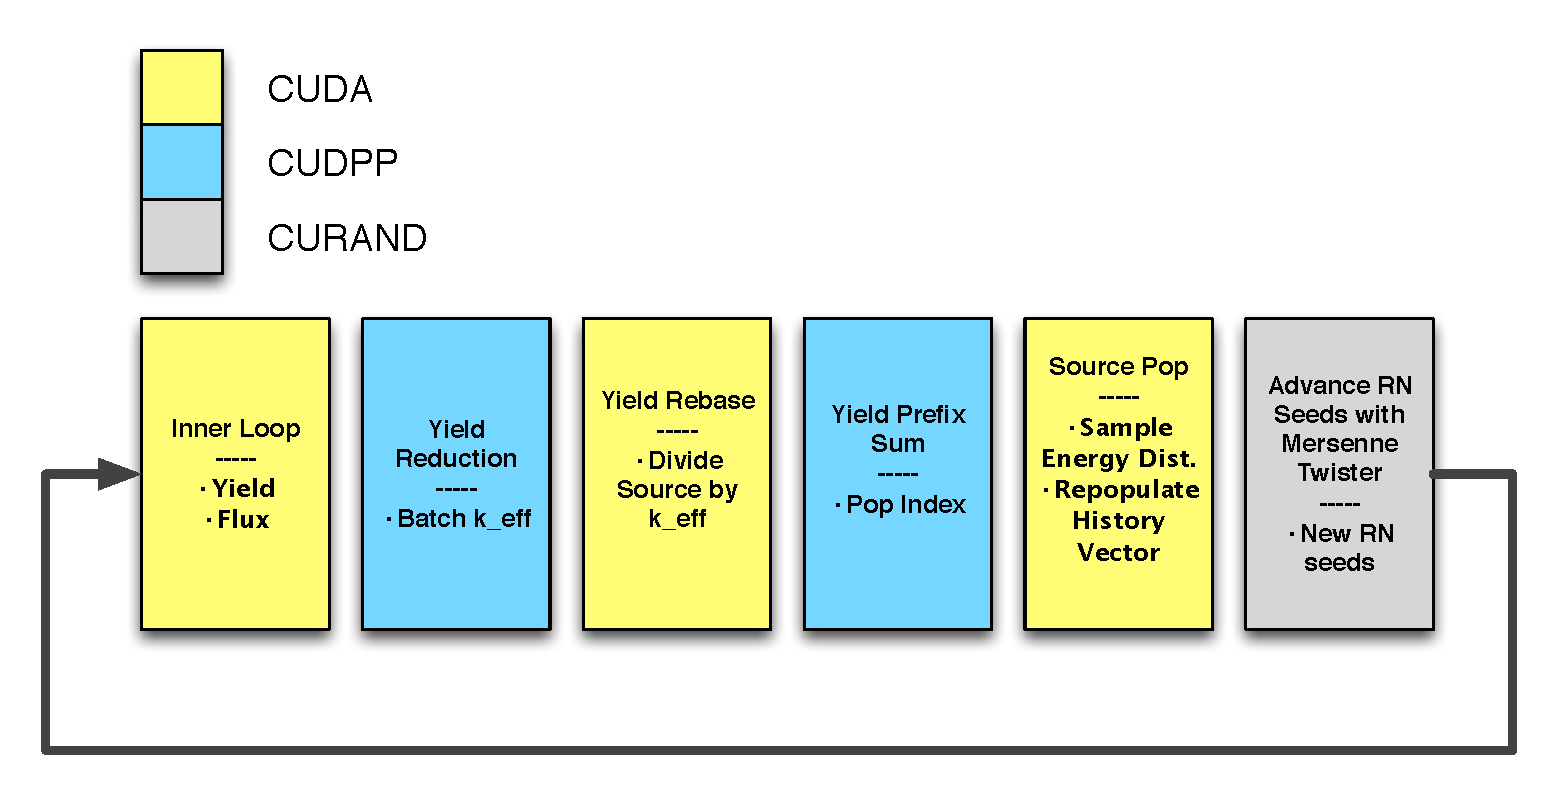
\includegraphics[width=0.9\textwidth]{graphics/warp_outer_loop.eps}
\caption{WARP outer transport loop that is executed in between neutron batches for criticality source runs. \label{warp_outer_loop} }
\end{figure}

Fixed source runs do not have an outer loop since the source is not dependent on the flux and does not need to be reconstructed based on the yields of the last batch.  If there is enough memory available, the entire number of requested neutrons are initialized based on the source definition.  The neutrons are transported simultaneously, and any secondary neutrons produced from fission or (n,2/3/4n) reactions are popped into the history vector at the end of the inner loop to be transported with the original source particles in the next pass of the loop.

\subsection{Grid Search Kernel}

Much effort has been done in order to require one search on the main unionized energy grid to find the index $i$ which satisfies $E_i<E<E_{i+1}$, but the best algorithm to do so has not been established.  It is convenient that the values in the energy grid are monotonically increasing, but since the array is composed of floating point values with arbitrary spacing, an inverse function cannot made to calculate an index in $O(1)$ time.   A naive approach would be to scan the array from be beginning, performing comparisons along the way, and therefore calculating the cross section array index in $O(n)$ time, where $n$ is the number of elements in the array.  This method does not scale well, however, and will not be considered.  

An extreme method taking advantage of the space-time tradeoff would be to use a simple lookup vector where the points are linearly spaced.  In order to include all original data, the spacing of the lookup vector, $dx$, would have to be smaller than the smallest found in the data.  The lookup vector index could simply be calculated by $i=E/dx$, and cross sections could be searched in constant time.  The spacing around resonances in the nuclear data is very small, however, and makes this method's memory usage unacceptable large.  For uranium-235, the smallest difference is $10^{-12}$ MeV over a range of $10^{-11}$ to 20 MeV, indicating that the vector would need to be around $20/10^{-12} \approx 10^{14}$ elements long.  Logarithmic spacing could also be used, but again assuring that all original data is included may make the regular grid too fine, resulting in unacceptable memory usage.

The binary search is the classic search algorithm for searching irregular data.  Instead of progressing through the array from start to end, it is continually bisected until the correct interval is found.  In other words, the search begins at the center of the vector.  If the searched-for value to less than the middle value, the next loaded value is the middle value of the first bisection.  If the searched-for value to greater than the middle value, the next loaded value is the middle value of the second bisection.  This process repeats iteratively until the value is found.  The binary search algorithm is attractive because it runs in $O(\log_2(n))$ loads/comparisons in the worst case, and uses no storage except for the loaded and comparing values \cite{something}.

Many methods were considered in the development of Serpent, most notably reconstructing the unionized dataset with a evenly-spaced grid whose indices could be calculated analytically.  The cross sections are linearly interpolated, or alternatively set to the lower point value (histogram method), between the new regular grid.  The reported effects introduce more uncertainty into the results since information is lost around tightly-grouped energy points at resonances, but allow quick search times.  The histogram method is equivalent to the lookup vector outlined previously, but without the constraint of including all the original data.  Another approach described in Serpent overlays a regular grid over the original unionized data which contains pointers to the cross section data within the interval.  With this structure, the small overlay bins are calculated analytically, and the points within are searched iteratively (with a binary search, presumably).  This method decreases search time and does not discard data, but many redundant points are included within the intervals, leading to increased memory usage \cite {jaakko}.   The data use problem in the second Serpent approach can be overcome by simply including the index boundaries within the interval instead of the entire interval itself.  This way the iterative search domain can be substantially reduced with an analytic function without much memory overhead.

The binary search might be inefficient in from a memory bandwidth standpoint since each thread needs to performa this search.  When access becomes much more sparse after the first few iterations of the algorithm, bandwidth is lost from accessing single floating point values in a uncoalesced manner.  Since \lstinline{float4} values can be loaded in a single transaction, it may make bandwidth sense to take advantage of them.  Instead of bisecting the data on each iteration, requiring only one value to be loaded, the data can be divided in fives if four values are loaded.  Such an algorithm would converge faster than a binary search and would use as much bandwidth as possible.  But since the algorithm now has four values, the index which corresponds to the values is not clear (in binary search it is simply whatever the current index is).  To resolve this, the search can be made into a linked list, where a second \lstinline{float4} vector is loaded containing pointers to the next \lstinline{float4} value vector.  Figure \ref{quad_tree} shows how a thread would traverse this data structure.  The lowest level of the tree holds the original grid values, and the tree is built bottom-up.  When the energy value satisfies $E_{j-1}<E<E_{j}$, where $j$ is the local node's \lstinline{float4} indices, the thread accesses the next \lstinline{float4} node located at pointer $p_j$.  This traversal is done iteratively until a null pointer is encountered, which signals that the final main energy grid index $i$ that satisfies $E_{i}<E<E_{i+1}$ has been found.

\begin{figure}[h!] 
\centering
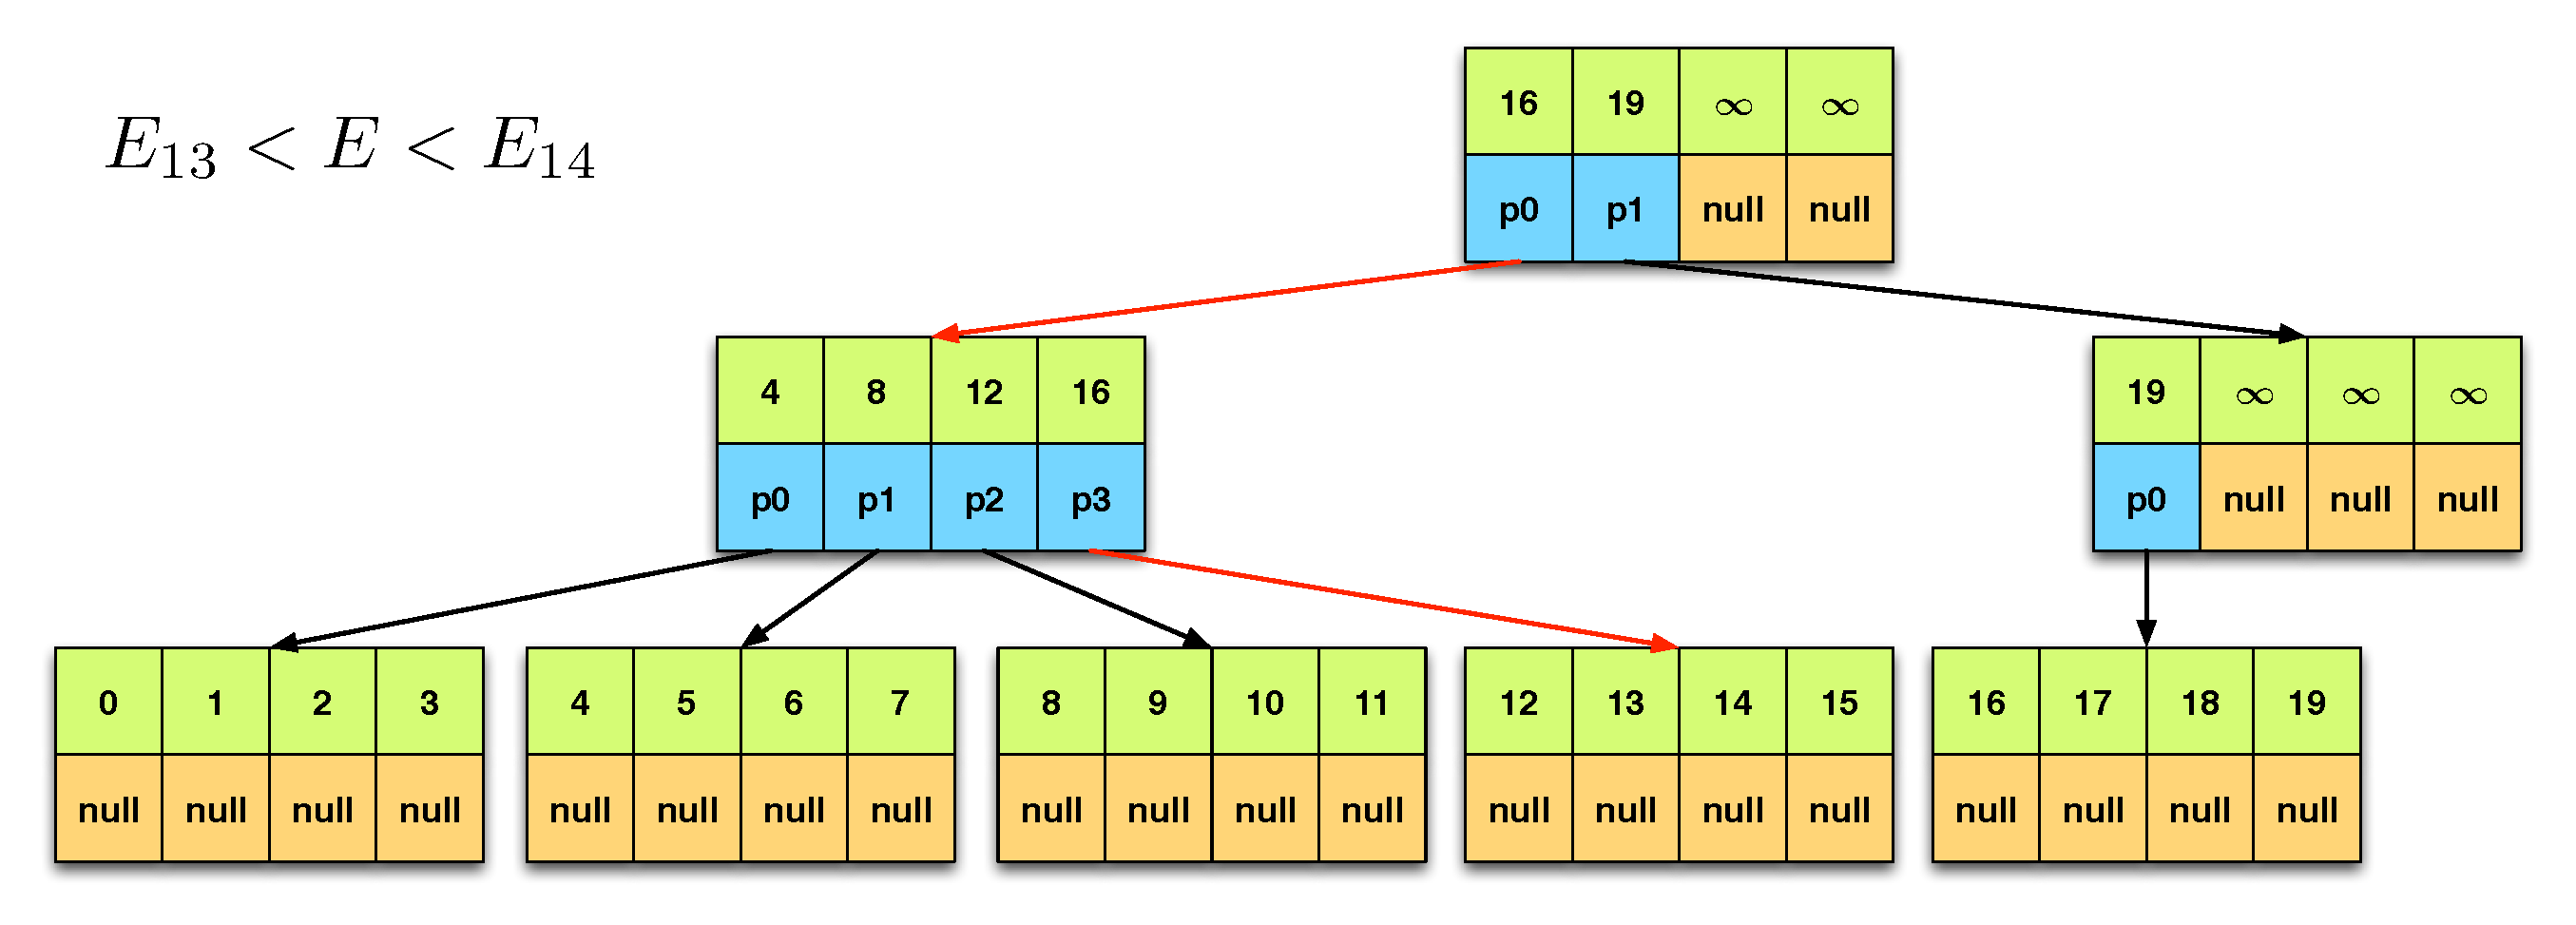
\includegraphics[width=1.0\textwidth]{graphics/quad_tree.eps}
\caption{A search employing a four-leaved tree structure where $E_{13}<E<E_{14}$. \label{quad_tree} }
\end{figure}

Another approach could be to use a high order polynomial approximation of the unionized grid for the initial guess of an iterative method.  This would be similar to the Serpent pointer search method, but would eliminate the pointer vector and use the analytical computation to find an initial index in the main grid instead of computing the index of the pointer vector.

WARP currently uses a simple binary search algorithm due to its logarithmic scaling and ease of implementation.  It will be determined if the grid search is a significant portion of the simulation time, and if it is, WARP could benefit by implementing more advanced searching algorithms in the future.

\subsection{Pseudo-Random Numbers}

Random numbers are the basis of the Monte Carlo method, and generating them must be done efficiently.  Since these numbers must be computed, they are not strictly random, but rather pseudo-random since they are randomly distributed but can be deterministically computed.  NVIDIA provides a random number library called CURAND which can generate large arrays of randomly distributed numbers.  Initially, WARP precomputed all the random numbers it would need for a single transport loop iteration.  This could be done since a direct sampling methods were used everywhere (which was incorrect for the target velocity in scattering) and there was a maximum number of numbers required.  The threads would simply access rand number values stored in this giant array (about 20 numbers were needed per thread).  This is a very bandwidth-intensive way to access random numbers since they are always written and read from global memory.  In these early implementations, the random number generation and access was taking about a quarter of the transport loop time.  In addition, the introduction of the correct rejection sampling method for the target velocity disqualifies precomputation since there no longer was an absolute maximum amount of numbers needed.

Taking these points into consideration, it was decided to use a linear congruential random number generator (LCRNG) for computing random numbers in the transport kernels.  It allows the kernels to generate random numbers with the recursion relations shown in \eqref{lcrng}, where $x_{n-1}$ is the previous random number.  The values $a$, $c$, and $m$ are taken from Pierre L'Ecuyer's manual for configurations with a high figure of merit \cite{lcrng}.   

\begin{equation}
\begin{split}
x_{n} &= a x_{n-1} + c \mod m  \\
a &= 116646453 \\
m &=  2^{30} \\
c &= 7
\end{split}
\label{lcrng}
\end{equation}

LCRNGs are based on integer numbers which must be converted to floats when the numbers are needed.  This is done by simply dividing my the modulus value $m$.  OpenMC uses a similar version, but since WARP uses single precision, different values were needed.   One was chosen close to the full 32-bit range for maximum floating point resolution.  Having a modulus as a power of two is very convenient as well since the modulus can be performed by bit truncation rather than a full modulus operation \cite{openmc}.  In other words, the operation can be done by a bitwise AND operation between $a x_{n-1} + c$ and $2^{30}-1$, which in binary is all ones below the 30th bit.

Using a LCRNG keeps global access down and improves performance greatly, since a single seed value is loaded at the start of the transport loop, stored in fast registers, then written back at the end of the loop.  CURAND is used outside of cycle to advance the seed bank with the Mersenne Twister algorithm (which has a period of $2^{19937} - 1$) to make sure no correlated numbers are used as intermediate seeds.

\subsection{Macroscopic Kernel}

The macroscopic kernel in WARP computes all values related to macroscopic cross sections.  These include total macroscopic cross section for the material, interaction distance, which isotope the neutron interacts with, moving the neutron to the nearer of the interaction/intersection distance, and setting the neutrons reaction number to the resample flag if the intersection is closer.  

Since the isotopes total cross sections are stored together in the unionized cross section matrix, the total macroscopic cross section can scan the contiguous row of this part of the matrix, interpolating the value between $i$ and $i+1$, which was found by the grid search kernel.  The interpolated values are multiplied the values by the atom density vector (in atoms/barn-cm, which contains a zero for isotopes not present) and the sum is accumulated as shown in \eqref{macro_vector}.  When the material vector has been completely scanned and total cross section is computed, the array is scanned again, but this time a random number is used to determined which isotope the neutron interacts with via \eqref{isotope_selection}.

\begin{equation}
\Sigma_t(E) = \sum_{k=0}^{N_\mathrm{isotopes}} M_k \: \Sigma_{t,k}(E)
\label{macro_vector}
\end{equation}

The material's total macroscopic cross section is also written to an array so the flux tally routine does not have to recompute it, which would take many more global memory transactions than loading it from the array.  Next, the interaction distance is sampled via \eqref{first_col_samp} and is compared against the nearest surface distance, which was computed with OptiX in the first step of the transport loop.  If the interaction distance is nearer, the neutron's coordinates changed to this location.  If the surface is closer, the neutron is moved to the surface and its reaction number is changed to the resample flag value, which will cause it to skip all other kernels until OptiX determines the new material and resets its reaction flag.

\subsection{Flux Tally Kernel}

The flux tally kernel simply scores the predefined tally bins via \eqref{flux_tally}.  Currently, WARP only allows evenly spaced logarithmic bins since their indices can be calculated analytically (as opposed to an arbitrary input grid).  The tally index $j$ out of $N_\mathrm{tally}$ bins for a neutron with energy $E$ is calculated via \eqref{tally_index}.  Since multiple threads could be adding to the element located at $j$, atomic operations are used to perform to sum, specifically the atomicAdd() function.  Atomic functions perform the load-compute-store operations in a single, uninterruptible transaction.  This eliminates the risk of data races occurring.

\begin{equation}
j = \mathrm{floor} \left( \frac{ \log \left( \frac{E}{E_\mathrm{min}} \right)} { \log \left( \frac{E_\mathrm{max}}{E_\mathrm{min}} \right)} (N_\mathrm{tally}-1) \right)
\label{tally_index}
\end{equation}

\subsection{Microscopic Kernel}

Unlike the macroscopic kernel, the microscopic kernel only has one job - to determine which reaction the neutron undergoes in the isotope it has been sampled to interact with.  This is done by scanning the isotope's subrow in the unionized cross section matrix as show in \eqref{micro_vector}.  $N_{\mathrm{start},k}$ is the starting index of the row for isotope $k$, $N_{\mathrm{end},k}$ is the index of its last reaction cross section, and $\sigma_{t,k}(E)$ is isotope $k$'s total microscopic cross section.  The starting and ending indices for an isotope are precomputed and stored in a separate array.  For most runs, this array and the material isotope density array can be stored in fast shared memory.

\begin{equation}
\begin{gathered}
m <  N_{\mathrm{end},k}\\
 PDF_m = \frac{1}{\sigma_{t,k}(E)} \sum_{z=N_{\mathrm{start},k}}^{z=m}  \sigma_{i,z}(E)
 \end{gathered}
\label{micro_vector}
\end{equation}

Once the reaction $m$ is sampled, the sorting routine is launches to remap data references and sweep completed histories out, then reaction kernels can be launched to carry out the individual reactions.

\subsection{Interaction Kernels}

There are only four reaction kernels since all disappearance reactions are taken care of in the radix sort.  That only leaves the three different kinds of scattering ((n,2/3/4n) reactions follow laws of continuum scattering but have a yield which is taken care of in the pop routine) and fission.  The scattering reactions change the direction and energy of the neutrons, and their distributions are sampled as outlined in Section \ref{sec:stat}.  Here is where the pointer array becomes useful.  The row $i$ and column $m$ of the unionized cross section matrix have been determined, and the scattering kernels simply need access these coordinates in the scattering and energy pointer matrices to load the appropriate distribution data.  No additional searching needs to be done.

\subsubsection{Concurrent Kernels}

As mentioned previously, the reaction kernels should never access overlapping data, so they can all be launched concurrently.  NVIDIA cards with a compute capacity of 2.0 and higher support up to 16 concurrent kernel launches.  This is done by submitting these kernel launches to nonzero execution streams by declaring additional streams to be present and passing the stream objects to the kernel launches as an extra launch parameter.  Kernels launched on different streams can be executed concurrently and their blocks can be interleaved, which is why it is very important for them to act on independent data.

Kernels launched without an explicit stream are launched on the default stream 0, which are are synchronous (program flow does not continue on the host until the launch is complete).  If kernel synchronization is important after execution completes (as it is here, reactions must be carried out before the OptiX trace), the streams must be synchronized with a an explicit stream synchronization command or with a synchronous operation like a cudaMemcpy().

\subsection{Parallel Operations}

The array-wide parallel operations in WARP are done with the CUDPP library.  The functions used are reductions for calculating $k_\mathrm{eff}$ via \eqref{k_eff_batch}, prefix sums for calculating the indices for the source pop kernels, and sorts for keeping warps coherent and full after the microscopic kernel.

\subsubsection{Remapping with Radix Sort}

Since the reaction numbers are integers, they can be sorted by very efficient algorithms like a radix sort which performs in $O(kn)$, where $n$ is the number of values to be sorted and $k$ is the number of significant digits of the values.  In WARP, there are less than 999 reaction types, so $k=3$.  The reaction number encodings in WARP are shown in Table \ref{WARP_numbers}.  Since reaction 999 represents a terminated particle, the sort will push all the completed history references to the end of the remapping vector.  Figure \ref{radix_sort} shows how the radix sort will arrange the remap vector and how threads will be mapped to the data.  CUDPP's radix sort conveniently sorts for key-value pairs, and WARP uses the reaction numbers as keys and the data index as values, effectively creating a remap vector.

\begin{figure}[h!] 
\centering
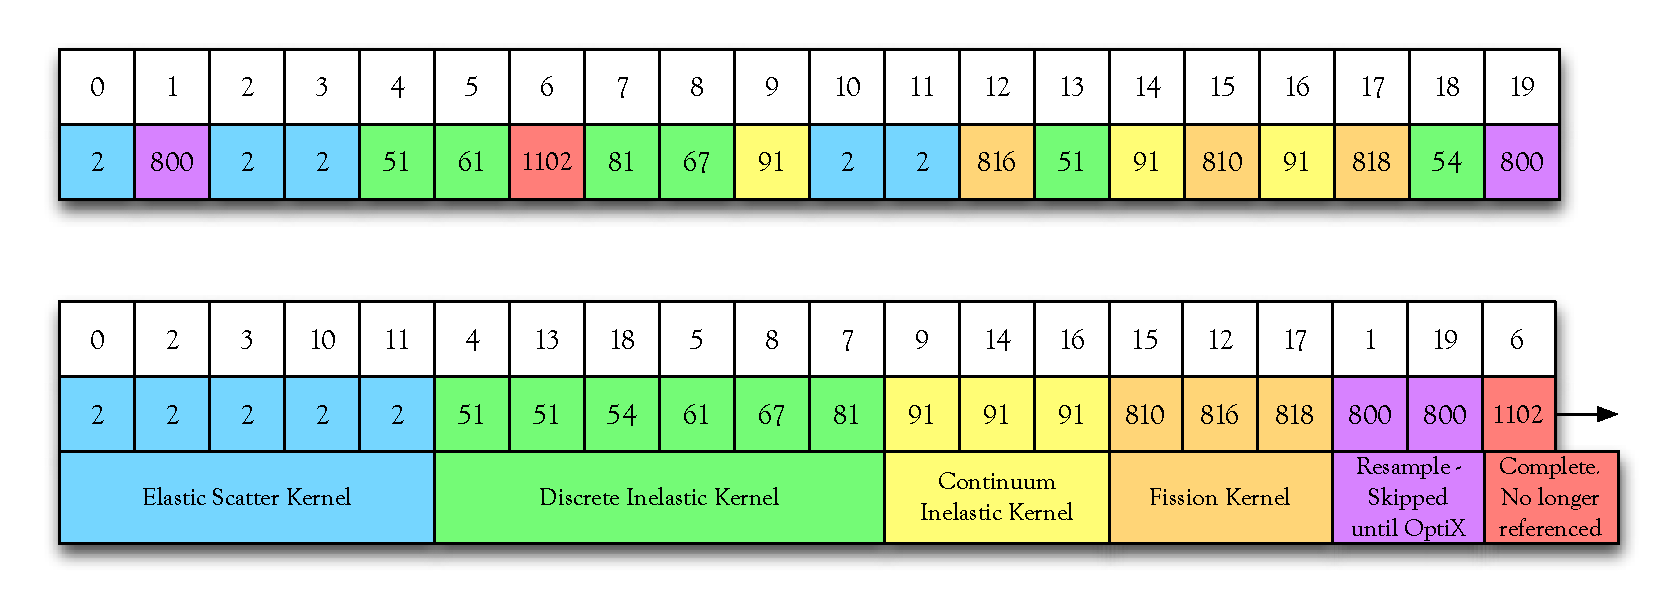
\includegraphics[width=1.0\textwidth]{graphics/radix_horiz.eps}
\caption{A radix key-value sort creating a remapping vector. \label{radix_sort} }
\end{figure}

There is one more piece of information that is needed to launch the reaction kernels concurrently - the number of particles undergoing each type of reaction.  This is determined by launching a comparison kernel on the sorted array which detects the places where the reaction numbers change.  The algorithm to do this is a simple adjacent comparison.  If there are $N$ elements in the array, $N-1$ threads are launched which load values tid and tid+1.  If the values are different, tid is the last index of a reaction type.  Since there are coarse boundaries for the reaction kernels, only 4 transitions need to be recorded can copied back to the host.  The groups are MT=2 for the elastic kernel, MT=18-21 and MT=38 for fission, MT=51-90 for discrete inelastic scattering, and MT=91 for continuum scattering.  Reactions with MT numbers larger than 91 do not produce secondary neutrons and are treated as capture.  MT=11-45 not including the fission numbers can usually be treated as continuum scattering (ENDF law 44), but may not be true for all isotopes.  Finer-grained reaction kernels may be a future development point of WARP.  If a launched thread lies on a boundary, it writes its index into a vector containing  10 elements, the start and end indices for the 4 reaction kernels (4 values are needed for continuum for its two blocks).  Since there is only two boundary for each reaction group, this can be done without atomic operations since only one thread should ever write to an element.  This vector is copied back to the host and used to calculated the number of blocks launched with each reaction kernel.  Terminated neutron data pushed to the end of the remapping vector will not be accessed by active blocks, eliminating the need for an absorption kernel.

\subsubsection{Criticality Source}

As was mentioned previously, when the simulation is run in criticality mode, the source points for neutron batches depend on the fission points in the previous batch.  But if $k_\mathrm{eff}$ is not equal to one, each source neutron no longer corresponds to a secondary neutron.  This is the same problem in the time-independent NTE, where getting rid of the time dependent term causes the equation to be inconsistent if the multiplication factor is not one.  To remedy this, the fission source term is divided by the multiplication factor to force the equations to be consistent (assuming the multiplication factor is known).  Similarly, the fission yield vector of a batch of neutrons can be renormalized to artificially make the multiplication factor equal to unity by rearranging \eqref{k_eff_batch} as shown in \eqref{k_eff_rebase} where $n$ is the batch number, $N_d$ is the length of the dataset, $y_j$ is the secondary neutron yield of particle $j$, and $N_f$ is the total number of secondary neutrons.

\begin{equation}
\label{k_eff_rebase}
\sum_{j=0}^{N_d}  \frac{y_j }{k_{\mathrm{eff},n}} = \frac{N_{f,n}}{k_{\mathrm{eff},n}} \Rightarrow N_{s,n+1} = N_{s,n}
\end{equation}

Since WARP handless all neutrons with equal importance, yields must be integers, but $y_j/k_\mathrm{eff}$ rarely will be.  Stochastic rounding is used to round $y_j/k_\mathrm{eff}$ to the lower integer with probability $y_j/k_\mathrm{eff} - \mathrm{floor}(y_j/k_\mathrm{eff})$.  Since yields range from 2-5 neutrons, there will be many individual instances of each original yield and in the entire dataset, and yields will approach the mean $y_j/k_\mathrm{eff}$.

Once the yield vector is rebased by dividing by $k_\mathrm{eff}$ and stochastically rounding to a nearest integer, a prefix sum is done on the yield vector.  An exclusive prefix sum, or exclusive scan as CUDPP calls it, contains the sum of all the array values before index $j$ at index $j$ as shown in \eqref{prefix_sum}.  Such a vector can be used in the pop kernel, which writes the secondary particle data into the next batch's initial data based on the yield vector.

\begin{equation}
p_n = \sum_0^{n-1} \: x_i
\label{prefix_sum}
\end{equation}

after the prefix sum is done, the source pop kernel is launched.  A thread is launched for every element of the history dataset, and If a thread encounters a yield value of zero, it returns.  If a nonzero value is encountered, the thread samples $y_j$ secondary particles and writes them into the history data from $p_j$ to $p_j+y_j$.  Since the yields have been rebased, this should either just fall short or slightly over the total dataset size, $N_d$.  Of course, the yield vectors are immediately set to zero for all particles in the next generation.

Having to keep generational information to determine $k_\mathrm{eff}$ and the next generation's source distribution forces criticality calculations to use a batch-like transport approach.  Transport on the GPU becomes inefficient when few active neutrons remain in the dataset.  Formulating a way where generations did not need to be run in series could benefit the GPU greatly.  A potential way would be to associate generational information to neutrons, transporting them as in a fixed-source problem, then post-processing the results to determine $k_\mathrm{eff}$. 

\subsubsection{Fixed Source \& Subcritical Multiplication}

In fixed source mode, the secondary particles can be popped back into the active particle dataset at the end of the inner loop since generational information is not needed and only the system response to the pulse is desired.  In this mode, the number of source neutrons is given as an input, and memory allowing, a dataset of source neutrons this size is made.  These neutrons and transported and any secondary-producing reactions are popped back into the actively transporting dataset.  This is done by performing a compaction operation on the \emph{completed} dataset indices and a prefix sum is done on the yield vector.  A pop routine is done similar to a criticality source run, but the threads with a nonzero yield write into the indices where a neutron has been terminated, which specified by writing into indices $p_j$ to $p_j+y_j$ of the compaction vector instead of $p_j$ to $p_j+y_j$ of the dataset itself.  This reactivates terminated particle data for transporting secondary neutrons.  Of course, the terminated neutron data is all replaced by data appropriately sampled for the secondary neutron reaction.  As mentioned previously, it is necessary to be subcritical in fixed source mode, or subsequent generations will grow instead of shrink and the total number of neutrons needing to be transported to calculate the response will diverge.


